\documentclass[12pt]{report}
\usepackage[utf8]{inputenc}
\usepackage{amsmath,fullpage,amsfonts,amssymb,tikz,booktabs,geometry,amsthm,pgfplots,relsize,graphicx}
\usepackage[boxruled]{algorithm2e}
\usepackage{multicol}
\usepackage{graphicx}
\usepackage[most]{tcolorbox}
\usepackage{subfig}
\geometry{margin=1in}
\usetikzlibrary{matrix}
\pgfplotsset{soldot/.style={color=blue,only marks,mark=*}} \pgfplotsset{holdot/.style={color=blue,fill=white,only marks,mark=*}}
\usepackage{hyperref}
\usepackage{setspace}
\doublespacing
\title{Exploring dynamic Hamiltonian Monte Carlo for Bayesian neural networks}
\author{Yiu Sing Lau}
\date{}
\begin{document}

\begin{titlepage}
    \begin{center}
        \vspace*{1cm}
        \Large
        \textbf{Exploring Dynamic Hamiltonian Monte Carlo for Bayesian Neural Networks}
        \normalsize
         
        \vspace{1.5cm}
        
        \textbf{Yiu Sing Lau} \\
        Master of Science \\
        Department of Mathematics and Statistics 
        
        \vspace{1.5cm}
        McGill University \\
        Montreal, Quebec
        August 2018

        
        \vfill
        
        A thesis submitted to McGill University in partial fulfillment of the requirements of  the degree of Master of Science\\
        
        \vspace{0.8cm}
        
        
        
        
        
    \end{center}
\end{titlepage}

\renewcommand{\abstractname}{ACKNOWLEDGEMENTS}
\begin{abstract}
I would like to thank my supervisor Dr.Stephens for being patient and understanding with me, and for providing much needed financial support. Also the financial support from the Department of Mathematics and Statistics of McGill University is much appreciated.
\end{abstract}

\renewcommand{\abstractname}{ABSTRACT}

\begin{abstract}
Neural network models have seen tremendous success in predictive tasks in machine learning and artificial intelligence, with some attributing their success to implicit use of Bayesian inference \cite{mandt2017stochastic}. Stan is a state of the art software for Bayesian statistical computing used mainly in the statistical community, however, it is not optimized for use with neural network models. In this thesis, we replicated much of Stan's No U-Turn sampler in PyTorch and explore its use for sampling from Bayesian neural network models. We were able to explore different samplers,model structures and their sampling and predictive performances, on a benchmark classification task. We found that Bayesian inference gives more robust predictive performance compared to their frequentist counterparts in general, but care is needed with the choice of prior and the MCMC sampler. 

\end{abstract}
\tableofcontents 

\chapter{Introduction}
In this thesis, we will examine the problem of Bayesian computation as it pertains to neural network models. There are two main themes in this thesis. The first is the Stan software, the HMC samplers implemented therein, the principles behind these samplers, as well as the diagnostic tools that come with it. The second are the Bayesian neural network models, which has been hugely popular in deep learning. Since we will use HMC samplers to sample from the posterior of the Bayesian neural networks, we would have to first understand the inner workings of these samplers. This motivates the order in which we chose to present these two themes.

\section{Stan}

Stan has replaced most Bayesian statistical softwares like JAGS and WINBUGS as the recommended tool for Bayesian inference requiring Markov Chain Monte Carlo (MCMC)  because of its effectiveness, relative ease to learn, clear and extensive documentation, as well as its large community of users and expert support staff. Roughly based on the No-U-Turn sampler (NUTS) \cite{hoffman2014no}, it has since evolved from the original NUTS sampler and has many more features built in to facilitate sampling and diagnosing sampling issues.

In Chapter 2, after giving a short introduction to MCMC, we will give an extensive overview of Hamiltonian Monte Carlo (HMC), which is the foundation on which NUTS is built. This is important for understanding why HMC is used for sampling from the Bayesian neural network models that we introduce in Chapter 3. 
Then we will explain the version of No U-TURN Sampler implemented in Stan, highlighting its difference from the original implemnted in \cite{hoffman2014no}. The exhasutive terminal criteiron for NUTS (XHMC) , which has not been exposed in the latest version of Stan yet, has been shown to improve sampling efficiency in correlated distributions.  \cite{betancourt2016identifying}. Experiments comparing its performance against the default termination criterion will be discussed in Chapter 4. Then we will review the automatic tuning strategies for the step size parameter and covariance metric used by Stan, followed by a discussion of the built-in convergence diagnostics, NUTS-specific and otherwise.
Finally, we discuss some of the numerical tricks used by Stan that are omitted in the official documentation but can be critical for creating a robust implementation. 

Most algorithms discussed in chapter 2 will come with clear pseudocode and have been implemented in Python. Source code will be provided.


\section{Bayesian Neural Networks}

Neural network models have become hugely popular under the name of Deep Learning, attracting a lot of attention from researchers and practitioners alike \cite{goodfellow2016deep}. Many of its successes come from applications in vision, text, speech, and many other sub-fields in the field of artificial intelligence. However, there is not yet a consensus that explains why these models do so well, in many cases defying existing learning theory. 


In Chapter 3 we give a brief overview of the Bayesian neural network literature and identify areas where we feel could benefit from new developments in NUTS and related sampling techniques. In Neal's and Cho's work \cite{neal2012bayesian,choo2000learning}, sampling from the posterior distribution was by alternating between the lower and higher level parameters in a block-Gibbs fashion. With the model and data they used, they found joint sampling worse than Gibbs sampling for sampling the hyperparameter. We found that NUTS is capable of sampling the hyperparameter quite well (Section \ref{sec:hyperparameter}) , is more robust to tuning parameters (Section \ref{sec:xhmc}), and requires much less manual tuning.

Then we talk about the choice of prior for neural network models. In the 1990s it was standard to put a hierarchical prior on the model weights , but in the new wave of Bayesian deep learning literature the standard normal prior is used most of the times. Recently shrinkage priors like the horseshoe prior have been used to automatically regularize the weights \cite{ghosh2017model}. In their paper the authors used variational inference to approximate the predictive distribution, which might miss important features of the  distribution. In Section \ref{sec:priors}, we used NUTS to perform full posterior inference on a range of shrinkage priors . In short, we found that the standard normal prior performed best in terms of both effective sample size and predictive accuracy. The results of these experiments in full details will be presented in Chapter 4.

While the use of shrinkage priors should eliminate much of the need for model selection: one would simply fit the largest model possible and let the shrinkage prior eliminate any excess capacity, in practice sampling from such a model might prove too difficult, for example having too many hidden layers might result in vanishing or exploding gradients \cite{bengio1994learning}. There are also tuning parameters, like the activation function, which can not be chose by shrinkage priors. This necessitates model selection techniques. Model selection by information criteria like AIC and BIC is not backed by theory because neural networks violate one of their regularity conditions, namely that the model must have non-singular Fisher matrix. The Watanabe Information Criterion (WAIC) is designed to overcome this problem for all singular models. We experimented with the WAIC but found that it failed to choose the model that minimizes the test error on the dataset we chose. 

We also experimented with Stochastic Gradient Hamiltonian Monte Carlo (SGHMC), a version of Hamiltonian Monte Carlo that only uses a fraction of the data to approximate the gradient of the full posterior density function. In \cite{betancourt2015fundamental} the author showed that stochastic gradients causes divergence in high dimensional problems and is not recommended. Our experiments show that SGHMC can yield better predictive performance than full HMC but it requires careful tuning and is not robust to the initial tuning parameters. 

Initialization strategies where the weights are sampled from a normal distribution whose variance is scaled by the number of incoming units have been widely adopted for improving the final predictive accuracy. It motivates one to use such scaled normal distributions as the prior distribution. Its impact on predictive accuracy and sampling quality will be discussed in Chapter 4. 

\chapter{Stan}
\section{Hamiltonian Monte Carlo}

Bayesian inference can be simply summarized by the specification of a likelihood and a prior function. Suppose $q \in \mathbb{R}^D$ is the $D$-dimensional parameter of the likelihood function for observed data $X \sim \pi(x|q)$, we can
model our uncertainty about it with a prior function $\pi(q)$. Upon observing the data, we can perform Bayesian inference by using information provided by the posterior distribution 

\[ \pi(q | x ) \propto \pi(x | q) \pi(q) ,\]
for example to carry out maximum a posteriori estimation (MAP) , marginal posterior estimation and to compute credible intervals. The exact calculation of the normalizing constant $Z = \int \pi(x | q) \pi(q) dq $ is possible for certain convenient functions only, and we must rely on Markov Chain Monte Carlo (MCMC) to calculate posterior quantities. 


The most basic form of MCMC is the Metropolis-Hastings (MH) sampler. Suppose we have a an unnormalized density $\pi(q)$, and $h(q,p)$ is a proposal function such that conditional on the current state $q$, the probability of moving from $q$ to a measurable set $A$ is denoted by $h(q,A)$, we can calculate the Hastings ratio
\[ r(q,q') = \frac{\pi(q')h(q',q)}{\pi(q)h(q,q')}. \]
Then we accept the move to state $q'$ with probability $ \min (1, r(q,q')) $.

\begin{algorithm}
\caption{Metropolis Hastings Sampler}
\KwIn{$q_0$ initial state, $\pi(\cdot)$ unnormalized target density, $h(\cdot,\cdot)$ proposal density}


\For{$i = 1:n$}{
  	Draw $q_{\text{prop}}$ from $h(q_{i-1},\cdot)$ \;  	
  	Accept $q_{\text{prop}}$ with probability $\min(1,r(q_{\text{prop}},q_{i-1}))$ \;
  	
}
 
 
\end{algorithm}


The use of MCMC in statistical applications began with \cite{geman1984stochastic,besag1986statistical} in the field of image analysis. Because of the high-dimensional nature of image datasets, initially only the Gibbs sampler was used, circumventing the well known slow-mixing/low-acceptance behaviour of the random-walk Metropolis-Hastings sampler in high dimensions. The introduction of Hamiltonian Monte Carlo into the field of statistics by Neal \cite{neal2011mcmc,neal2012bayesian}, who built on the work of physicists using HMC to simulate from lattice field models \cite{duane1987hybrid}, brings an exciting new tool that allows statisicians to simulate much more efficiently from high-dimenisonal distributions. Unfortunately, because of the relative difficulty in implementing such samplers its use in statistics has been limited. In the last few years there has been a rebirth of the HMC sampler, with new developments that try to utilize information about the local curvature of the density function during  sampling \cite{girolami2011riemann,betancourt2013general}, as well as  automate the selection of tuning parameters.  \cite{hoffman2014no,betancourt2016identifying}. 
Arguably the most important development that is part of this rebirth is the development of the No U-Turn Sampler and the Stan software which uses NUTS as its main sampler. We also have a better theoretical understanding of the HMC with works \cite{betancourt2014geometric,livingstone2016geometric}
that provides a differential geometric interpretation of the sampler and conditions under which geometric convergence can be obtained.

First we give a brief introduction to the HMC, explaining the algorithm and listing its major features and advantages. 

Suppose we have a density $\pi(q),q \in \mathbb{R}^D$ from which we would like to
sample. If $\pi(q)$ is simply the marginal density of some distribution $\pi(q,p),
(q,p) \in \mathbb{R}^{2D}$ in a larger space containing the original domain, then sampling from $\pi(q,p)$ and keeping only the $q$'s is equivalent to sampling from $\pi(q)$ directly. These extra variables introduced are called auxillary variables. Auxillary variable methods are known to speed up sampling by introducing extra degrees of freedom in the state space and allows the chain to move more easily across different parts of it. The Swendsen-Wang sampler \cite{wang1990cluster}, the slice sampler\cite{wang1990cluster} are well known examples of this class of methods. See \cite{liang2011advanced,liu2008monte} for more details.

The Metropolis-Hastings sampler introduced above is a general algorithm that allows us to sample from any distribution, discrete, continuous or neither, as long as we know its density up to its normalizing constant. The Hamiltonian Monte Carlo (HMC) sampler is a particular class of MH sampler that requires the unnormalized density to be continuous and differentiable. It is also an auxiliary variable method. 


We denote the unnormalized density of the target distribution by $\pi(q)$, and the normalizing constant by $Z = \int\pi(q)dq $, and define the potential energy function $V(q)$ as 
\[ V(q) =  -\log \pi(q) .\]
If we now introduce a kinetic energy function $T(p)$, and define
the Hamiltonian as the total energy, i.e., sum of the kinetic and potential energy functions, 
\[ H(q,p) = V(q) + T(p) \]
we get that 
\[\pi(q,p) \propto  \exp(-H(q,p)) \]
has $\pi(q)$ as the marginal density, and thus defines an auxiliary variable method. In keeping with the physical analogy the auxiliary variable is usually labelled as the momentum.  In statistical applications, we usually have $\pi(q)$ as the unnormalized posterior
density, 
\[V(q) = -\log(\text{prior}(q) \cdot \text{likelihood}(q|data) ), \]
and 
\[T(p) = \sum_{i=1}^D \frac{p_i^2}{m_i}, \]
which is equivalent to introducing an independent multivariate Gaussian random variable of
the same dimension as the original distribution as an auxiliary variable. Suppose the original distribution is of dimension $D$, then the auxiliary variable is also of dimension $D$. and the $i^{\text{th}}$ variable is a Gaussian random variable of mean 0 and variance $m_i$.

Note that there is a physical interpretation of the system. The Hamiltonian uniquely determines the motion of a particle, whose position in space at any time is described by the $q$ coordinates, and whose momentum is described by the $p$ coordinates. Its motion can be described by solving a system of ordinary differential equations in Hamiltonian dynamics, known as Hamilton's equations:
\begin{align*}
    \frac{dq}{dt} &= \frac{\partial H}{\partial p } \\
    \frac{dp}{dt} &= -\frac{\partial H}{\partial q}.
\end{align*}

To simulate the trajectory of a particle given its initial state $(q_0,p_0)$ one
would have to solve Hamilton's equations. Unfortunately, there are in general no
explicit solutions for Hamilton's equations except for trivial models. One would
then have to resort to numerical methods that discretize the Hamiltonian
dynamics \cite{leimkuhler2004simulating}. The discretization should
possess some nice properties, including reversibility and volume-preservation, to ensure convergence to the target distribution, as well as  maintain 
stability and accuracy of the approximation over long trajectories, the lack of which significantly reduces the efficiency of the sampler, irrespective of model-related factors which might affect sampling efficiency, like parametrization or posterior correlation.  

For the simple version of HMC where the momentum variable is independent from the position variable, i.e. $\pi(p|q)=\pi(p)$, an easy-to-implement integrator which is both volume-preserving and reversible, with lower approximation error than conventional alternatives for numerically solving differential equations, like Euler's method, known as the leapfrog integrator \cite{leimkuhler2004simulating}, exists and works as follows. At time $t$ of the trajectory, given its current position and momentum, $q(t)$ and $p(t)$,and step size $\epsilon$, we would update the position and momentum at time $t+\epsilon$ by setting 
\begin{align*}
    &p\left(t+\frac{\epsilon}{2}\right) = p(t) - \frac{\epsilon}{2}\cdot \frac{\partial
    U}{\partial
    q}q(t) \\
    &q(t+\epsilon) = q(t) + \epsilon  \frac{\partial K}{\partial p}\left(p\left(t+\frac{\epsilon}{2}\right)\right)
    \\
    &p(t+\epsilon) = p\left(t + \frac{\epsilon}{2}\right) - \frac{\epsilon} {2} \cdot \frac{\partial U}{\partial
    q}(q(t+\epsilon)).
\end{align*}

One leapfrog step consists of first a half-step update for momentum, a full-step
for position, then another half-step for momentum. Since the update for momentum
at time $t+\epsilon$ and time $t+\epsilon + \frac{\epsilon}{2}$ both involve
$q(t+\epsilon)$,  we can combine the updates in the implementation, so that instead of performing two half steps for momentum $p(t+\frac{\epsilon}{2}) \rightarrow p(t+\epsilon)$, then $ p(t+\epsilon) \rightarrow p\left(t+\epsilon + \frac{\epsilon}{2}\right)$, we can perform a full step for momentum $p(t+\frac{\epsilon}{2}) \rightarrow p(t+ \epsilon + \frac{\epsilon}{2}) $ as 
\begin{align}
p\left(t+\epsilon + \frac{\epsilon}{2}\right)  
&= p(t+\epsilon) - \frac{\epsilon}{2} \frac{\partial U}{\partial q }(q(t+\epsilon)) \\
&= p\left(t+\frac{\epsilon}{2}\right) - \frac{\epsilon}{2} \frac{\partial U}{\partial q }(q(t+\epsilon)) - \frac{\epsilon}{2} \frac{\partial U}{\partial q }(q(t+\epsilon)) \\
&= p\left(t+\frac{\epsilon}{2}\right) - \epsilon \frac{\partial U}{\partial q }(q(t+\epsilon)).
\end{align}

Note, however, we still need $p(t+\frac{\epsilon}{2})$ to perform the full
steps, so that at least one half step has to be made for the momentum. Also, in
this alternative implementation of the leapfrog integrator, momentum $p$ is
always one half step ahead of position, hence the last update for momentum has
to be a half step so we end up with $p(t+\epsilon L)$ and $q(t+\epsilon L )$,
both synchronized. The two implementations yield exactly the same updates, bar
loss of accuracy from calculating the sums and extra computer time for updating
the momentum variables twice in the naive implementation. 

Starting at some initial time $t_0$, with initial coordinates $(q(t_0),p(t_0))$, the position and momentum at time $t+s$ can be determined by repeating the steps above roughly $s/\epsilon = L$ times, taking care to round up or down. 

One advantage of the leapfrog integrator over other more well-known methods for
solving ODEs numerically such as Euler's method is that it is symplectic, which
means it preserves volume in the phase space. This
contributes to its relative stability along the trajectory compared to Euler's
method and its modifications. An unstable trajectory as simulated by Euler's
method would propose a state that has diverged from the energy level set to
which the initial state belong, which makes proposals much more likely to be
rejected, especially in high dimensional distributions.  However,
the leapfrog method does not preserve the Hamiltonian, so the energy of the particle would
oscillate as it is being simulated. It has important implications for the
sampling algorithm. Intuitively, this breaks the law of conservation of energy
and suggests the position of the particle at the end of its trajectory may
deviate from the correct trajectory, on which the energy should be preserved.
Reducing the step size would mitigate the problem but it comes with increased
computational costs. This necessitates the introduction of a Metropolis
acceptance step in order to preserve the invariant distribution. To explain
this, we shall put HMC in the context of an auxiliary variable method. 

First, the joint distribution of the position (original) and momentum(auxiliary)
variables is factored into a product of a conditional distribution $\pi(q,p|E)$ and an
independent marginal distribution $\pi(E)$, where $E$ is the Hamiltonian energy for the state $(q,p)$,
\[ \pi(q,p) = \pi(q,p|E)\pi(E) .\]

Sampling from the joint distribution is done by first sampling from the
auxiliary (energy) distribution $\pi(E)$. In this case randomness is introduced only during  the
re-sampling of the momentum variable, that is, change in the kinetic energy,
because the potential energy is not dependent on the momentum. Then, conditional on the value of the
current energy, we sample from the joint
conditional distribution of the position and momentum variables $\pi(q,p|E)$. Leapfrog steps
are involved only when sampling from the conditional distribution $\pi(q,p|E)$.
This "sampling" is actually deterministic as it consists of simulating a
trajectory under Hamiltonian dynamics with given initial states. Because
Hamiltonian flow is reversible and volume-preserving independent of numerical
discretization, convergence of the MCMC samples to the target distribution is guaranteed without the need for Metropolis
correction if we can simulate Hamiltonian dynamics exactly. Indeed, there has
been experiments with HMC where the Metropolis acceptance step is dispensed with
and samples drawn from the resulting algorithm, when used for inference, still yields good predictive
performance on regression tasks \cite{neal2012bayesian}, although it is offset
by
decreased robustness as the uncorrected trajectory could become unstable when
the step size becomes too large.
 
Now, we describe a simple version of the HMC sampler.
The sampler starts by drawing from the conditional (marginal because of
independence) distribution of the momentum/auxiliary variables $p$, then it simulates the
movement of a particle having initial position and momentum $(q,p)$ according to
Hamiltonian dynamics. More precisely, we do $L$ leapfrog steps of step size
$\epsilon$, both of which are important tuning parameters to the algorithm.
At the end of the trajectory we get $(q(t+L \epsilon),p(t+L \epsilon)) =
(\tilde{q}, \tilde{p})$, which becomes the proposed state for the chain and
is used in the calculation of the Hastings ratio. The proposed state is then accepted with probability $\min (1, \exp(H(t+L\epsilon)-H(t)))$. 


\begin{algorithm}
    \KwData{Input: potential energy function $V(q)$, its gradient $\nabla V(q)$, initial position $q_0$, $\epsilon$,$L$,$\Sigma$} 
    $q = q_0$ \;
    $p = \mathcal{N}(0,\Sigma)$ \;
    $p_{c} = p$ \;
    \For{$i = 1:L$}{
    $p = p - \frac{\epsilon}{2} * \nabla V(q)$ \;
    $q = q + \epsilon * \Sigma^{-1} p $ \;
    $p = p - \frac{\epsilon}{2} * \nabla V(q)$ \;
    }
    $p = -p $ \;
    $H_{c} = V(q_0) + \frac{p_c^T\Sigma^{-1}p_c}{2}$ \;
    $H_{n} = U(x) + \frac{p^T\Sigma^{-1}p}{2}$ \;
    $u  = Unif(0,1)$ \;
    \eIf{ $u < \min(1,\exp(H_{c} - H_{n}))$ }{
        $out = q$ \;
    }{
        $out = q_0$ \;
     }
\caption{HMC update}
\end{algorithm}

Here we state some facts about Hamiltonian dynamics that would help us
understand why proposals generated from the simulation of Hamiltonian dynamics would
form a Markov Chain sampler that has the right invariant properties. 

First, the Hamiltonian flow, i.e. the mapping induced by the Hamiltonian
dynamics, is reversible. That is, any mapping $T_s(q(t),p(t)) =(q(t+s),p(t+s)) $
is bijective and has an inverse $T_{-s}$. Intuitively, it says that any particle
whose trajectory follows Hamiltonian dynamics can be returned to its initial
state $(q_0,p_0)$ from current state $(q_t,q_t)$ by reversing the sign of $q_t$
and having the particle follow its trajectory for time $t$. Reversibility is
important as one of the necessary conditions for Markov Chains to have the
correct invariant distribution and
convergence properties \cite{robert2013monte}. 

Second, the Hamiltonian flow $T_s$ is a volume-preserving mapping. That is, 
\[ \text{Vol}(T_s(A)) = \text{Vol}(A), \]
where $A$ is a measurable set in the augmented parameter space (e.g.
$\mathbb{R}^{2d}$) which contains
the support of 
the joint probability density $\pi(q,p)$, and $Vol(\cdot)$ a volume measure. 
It makes it
possible to calculate the Hastings ratio without involving the determinant of
the Jacobian matrix of the mapping $T_s$, which might be tricky for most
mappings. For Hamiltonian flows the determinant is just one.
Third, the Hamiltonian is constant with respect to time, i.e., $\frac{dH}{dt} =
0$. From the physics point of view, this is simply the conservation of energy in
a closed system. It keeps acceptance probability high if the discrete simulation
of the Hamiltonian dynamics is accurate enough, which is equivalent to staying
close to the true trajectory, usually achieved by using a small leapfrog step size. This has been mentioned earlier
and we will look at it from another angle here. The Metropolis acceptance step
accepts the proposed state $(q_t,p_t)$ as the next state in the Markov chain
with probability $\min(1, \exp(-H(q_t,p_t) + H(q_0,p_0)))$, where $(q_0,p_0)$ is
the previous state in the chain, also the initial state in the Hamiltonian
trajectory. In theory, because we are sampling from an energy level set 
\[ S=\{(q,p)|H(q,p)=E\} \]
for some fixed energy value $E$, the entire trajectory
$(q_0,p_0),(q_\epsilon,p_\epsilon),\dots (q_{\epsilon L},p_{\epsilon L})$ where
$\epsilon L = t $ has the same Hamiltonian value $H(q_s,p_s)$. Then 
\[ -H(q_t,p_t) + H(q_0,p_0) = 0 \]
and the proposed state is accepted with probability 1. When a numerical
approximation to the correct Hamiltonian dynamics is used to find the proposed
state, it inevitably deviates from the exact trajectory, and the order of that
error determines how large the difference $ -H(q_t,p_t) + H(q_0,p_0)$ will be.
Although it is possible that $(q_t,p_t)$ gives a smaller energy that the initial
state and hence resulting in an acceptance probability of 1 as well, empirical
evidence suggests that the Hamiltonian tends to oscillate along the trajectory
traced out by leapfrog, and hence it is equally likely for $\exp(\Delta H)$ to be
larger or less than 1. 

Having discussed the Hamiltonian function, we now look at one of its two
components, the kinetic energy function $T(p)$.  Because the
Hamiltonian function remains constant along its trajectory after the initial
position and momentum is fixed, the only change in the value of the joint probability
density function $\pi(q,p)$ comes from the initial re-sampling of the momentum variables $p$
from its marginal distribution.

From the theory of auxiliary variable sampling we see that there are infinitely
many marginal distributions for the momentum variable $p$ that would give the
same target marginal distribution for the original parameter $q$. For example,
if we restrict 
\[ p \sim \mathcal{N}(0,M), \]
where the mass matrix $M$ is positive definite then any choice of $M$ on the support gives a
different kinetic energy and, by extension,a different Hamiltonian function. In the HMC
literature, the focus has been on Gaussian kinetic energies, 
justified by empirical performance and intuition appealing to the central limit
theorem. In \cite{girolami2011riemann} the authors experimented
with the more heavy-tailed Student-T distribution and found it to perform not as
well
as Gaussian momentum distributions. For the rest of the discussion of HMC we
assume a Gaussian distribution is used to model the auxiliary momentum variables.

A clever choice of mass matrix can significantly speed up the sampler. Its
selection mainly has to do with decorrelating the irregular geometry of the
target distribution,which slows down sampling. For example, if we would like to sample from a multivariate
highly correlated Gaussian distribution, one could adopt an
appropriately adjusted mass
matrix $M$ for the kinetic energy, and the induced sampling can be shown to be
equivalent to sampling from a standard Gaussian with identity covariance in a
linearly transformed parameter space. Sampling efficiently from a standard Gaussian
distribution is easy
for HMC and Random Walk Metropolis, because all the variables are independent and on
the same scale. Dimensionality has no impact on sampling in this case because
each dimension is sampled independently and separately, and since the proposal
distribution is Gaussian it is easy explore the support of the target
distribution as it overlaps with the target distribution
exactly. 

To see how to transform the problem of sampling from a skewed multivariate
Gaussian distribution to sampling from a standard Gaussian, let $q' = Aq$, where $A$ is an invertible matrix. If we also
transform the momentum variables $p' = (A^T)^{-1}p$ ,then the
Hamilton's equations for the transformed variables $(q',p')$ will be the same as
the original variables $(q,p)$. As an aside, note this also implies that HMC is rotationally
invariant, i.e. if $A$ is orthogonal, $A^{-1} = A^T$, then reparametrizing the
variables by  multiplying $(q,p)$ by $A$ would result in exactly the same simulated
trajectories if we keep all tuning parameters the same.

Suppose we want to sample from $q \sim \mathcal{N}(0,\Sigma)$. Let $p \sim
\mathcal{N}(0,\Sigma^{-1})$, then the updates would be equivalent to using an
identity covariance for $p$ for drawing from a standard multivariate Gaussian
distribution. This
fact about HMC suggests it would improve sampling efficiency if one has
access to the covariance of the target distribution and its inverse, although this is true for
MCMC sampling in general as well. 
In general the momentum distribution can be tuned by first exploring the density
with a simple HMC sampler with standard Gaussian momentum distribution, then use
the samples to estimate the covariance matrix of the target distribution, the
inverse of which could be set as the covariance.  For reasons of memory and time constraints it might be beneficial to use only the diagonal covariance. 

There are several reasons why HMC is better than random-walk Metropolis. First,
it avoids random walks in the parameter space. Random walks are inefficient because successive
proposals might double back to previous positions, thus limiting the range of
the exploration of the support, whereas Hamiltonian trajectories would be in the
same direction for many steps. Assuming independence, $n$ steps of random walk
would result in a random displacement of $n$ units. Its variance  
is a linear function of $n$. Its standard deviation is $O(\sqrt{n})$, and can be
interpreted as the typical distance a random walk moves. As an analogy, if we
have a 1-dimensional random walk $e_i \sim \mathcal{N}(0,\sigma^2)$ starting from
the origin, then,  with high probability the particle will end up in the
interval $(-\sqrt{\sigma},\sqrt{\sigma})$. 
On the other hand, since leapfrog steps are deterministic given initial position
and momentum, the distance moved will be proportional to $n$. 
Second, HMC is much more efficient in
high-dimensional settings. Because Random Walk Metropolis randomly proposes changes in
the $2^D$ possible directions, it becomes exponentially more unlikely to move
to an area of the support where there is significant mass. The acceptance
probability would be extremely low and the chain becomes stuck. On the other
hand, because HMC uses information of the gradient and an auxiliary variable
tuned to the curvature of the target distribution, the exploration stays close
to the mode and the high density neighbourhood around it. There is a delicate
balance between staying close to the mode and in the neighbourhood containing
the mode. From almost any standard introduction to statistical learning \cite{friedman2001elements} we learn about the curse of dimensionality, which says that the probability mass in the neighbourhood containing the mode of the density function decreases exponentially as the dimension increases. This means that simply sampling from around the mode will miss a lot of the support which contributes to the integral, but it remains an important starting point because the interesting part of the support lies just outside the immediate neighbourhood of the mode. The gradient draws the
trajectory to
the mode while the momentum variable keeps it from getting stuck there and moves it around with each resampling.



We have described some of the advantages of HMC, but unfortunately it has one great disadvantage, which is its sensitivity to tuning parameters. 
In the description of the basic HMC sampler above, we assume the step size $\epsilon$, trajectory length $L$, and the momentum covariance $M$ are known. These cannot be set arbitrarily as the performance of the algorithm can change completely when they are not set appropriately \cite{neal2011mcmc}. HMC can perform no better than random walk Metropolis -- itself an highly inefficient sampler -- for high-dimensional distributions. The manual tuning of these parameters is the next part of our discussion. 

The first parameter we will discuss is the step size $\epsilon$. A small step size would cost more computation time but gives better approximation to the correct trajectory. Worse still, when a too large step size is used, there are no constraints on how far the simulated trajectory would deviate from the correct one. The simulated trajectory could quickly move to a region of the support where the Hamiltonian function blows up. There needs to be a mechanism in the algorithm to detect divergence due to the step size and signals us to possibly tune it down, otherwise the unstable trajectory would diverge to infinity in terms of its Hamiltonian function value and causes the program to crash, not to mention a chain with too many divergences would generally be biased. It is suggested by Neal that introducing a random jitter around the step size at the start of each trajectory, for example, use $\epsilon + \epsilon*\text{Uniform}(-0.1,0.1)$ instead of $\epsilon$,  would help alleviate the problem, as sometimes the trajectory would be simulated using a step size under the stability limit for $\epsilon$, which can differ between different parts of the support of $\pi(q,p)$. This also deals with the problem of accidentally have $\epsilon L$ match the period of some variable or equivalently simulate a trajectory which returns to the original position at the end of its trajectory. This destroys ergodicity and makes the sampler biased. 

The second parameter of interest is the trajectory length $L$. Once $\epsilon$ is fixed, it is essentially a proxy for the integration time $t= \epsilon L$. It controls how much of the state space is explored at each iteration of the Markov chain. The longer we let the trajectory run the more of the state space would be explored, but letting it run too long we would eventually come back to the initial position and the exploration is wasted. Similar to the discussion about tuning $\epsilon$, the tuning of $L$ could be dependent on the part of the state space where the chain finds itself. In the basic HMC sampler, we use the same $\epsilon$ and $L$ throughout the entire sampling process.  

Neal \cite{neal2012bayesian} suggests doing several preliminary runs with a combination of $\epsilon$ and $L$ values using the acceptance rate as guidance. There is no guarantee of optimality and in even moderately complex distributions we never know whether we have sufficiently integrated the trajectory long enough. The optimal acceptance rate for HMC has been derived as $0.65$. Optimality here is defined with respect to the cost of obtaining an independent point. See \cite{neal2011mcmc} for an intuitive derivation and see \cite{beskos2013optimal} for a theoretical derivation. This sort of manual tuning is similar in spirit to the manual tuning strategies from the MCMC literature, and shares with them the disadvantage of requiring human intervention after each chain is sampled. 

A heuristic for manual tuning was given by Gelman et al.
\cite{gelman2014bayesian}: first fix $\epsilon L = t$, then adjust $\epsilon$
and $L$ by setting $\epsilon = \frac{\epsilon}{10} $ and $L = 10L$ and see the
changes reflected in diagnostics such as $ESS$ and trace plots. Of course, one
problem with this heuristic is that it fixes the integration time at $1$, which
might be too long or too short, depending on the contour of the target. The hand-tuning process can be made somewhat more efficient by listing all feasible values
for $\epsilon$ and $L$ and select the best combination by performing a grid-search. This only works if we accept
the use of a one-dimensional diagnostic to quantify the quality of samples
generated from a pair of $\{\epsilon,L\}$ values. This can be done by Bayesian
optimization as well. Whether selected by hand-tuning or Bayesian optimization,
the tuning process has no impact on the ergodicity of the sampler as we only
use the samples generated once we have decided on a pair of tuning parameters
$(\epsilon,L)$. This approach does not utilize information about the target
distribution, relying only on inappropriate choices of parameters to be weeded
out when the diagnostics indicate poor results.




So far we have already touched upon the integration time in discussion of
its connection with step sizes and trajectory lengths. It is a tuning parameter
that exists in both the theoretical and numerical version of HMC. In the
theoretical version, we assume Hamiltonian dynamics can be simulated exactly,
even then we would still have to decide the duration for which the imaginary
particle is integrated. This
is the amount of time we decide to simulate the trajectory in the augmented
space $(q,p)$ before projecting back to the sample space $(q)$. In any
numerical implementation this is subsumed in the product of the step size and the
number of leapfrog steps $\epsilon L$. It influences mainly the exploration of
the augmented space, where a trajectory is simulated along the level set
$\{(q,p):H(q,p)=E\}$.





\section{No U-Turn Sampler}


There exists an extension of the basic HMC sampler that seeks to increase the acceptance
rate by, conditioning on an initial state, proposing a state uniformly sampled over the leapfrog trajectory instead of always proposing the state at the end
of the trajectory. Two trajectories are proposed, one containing the initial state; one
of the two trajectories is chosen, then a state is sampled from the chosen
trajectory. The HMC update step is then much more likely to propose and accept
a state different from the initial state. This is Neal's window
method \cite{neal1992improved}. 

First we select a window size $W < L$, then sample randomly $s \in \{0, 1,2 , \dots , W -1 \}$. Take the current $(q,p)$ as $(q_s, p_s)$, we generate the sequence $[(q_0,p_0),(q_1, p_1), \dots (q_L,p_L)]$ stochastically by applying forward leapfrog steps (original leapfrog step with step size $\epsilon$) for $(q_i,p_i), i > s $, and backward leapfrog steps in random (step size equal to $-\epsilon$. ). 
Then the acceptance window is the sequence of $W$ $(q_i,p_i)$ pairs at the end of the trajectory, more specifically,

\[ \{(q_{L-W+1},p_{L-W+1}), \dots , (q_L,p_L)\}.\]

And the rejection window is the $W$ pairs 
\[ \{(q_0,p_0), \dots, (q_{W-1},p_{W-1})\}. \]

Then we set the probability of accepting the acceptance window as 

\[ \min (1, \frac{\sum_{i\in A} \pi(q_i,p_i)}{\sum_{j \in R} \pi(q_j,p_j) }) = \min (1, \frac{\sum_{i=L-W+1}^L \pi(q_i,p_i)}{\sum_{i=0}^{W-1}\pi(q_i,p_i)}), \]
where $A,R$ are the set of indices for pairs belonging to the acceptance window and rejection windows respectively. We are essentially choosing the acceptance window with probability equal to the ratio of the sum of probabilities of each pair in the acceptance window to the sum of probability of pairs in the rejection window. This is reminiscent of the Hastings ratio in standard Metropolis Hastings samplers. One can conceptualize this sampler as performing MH sampling over an augmented space where each state is a window of $W$ points in the original phase space.

Once a window has been chosen, we select a pair among the $W$ pairs in the window with probability weighted by $\pi(q_i,p_i)$. That is, suppose the rejection window is chosen, we chose the new state to be $(q_i,p_i)$, $i \in {0,\dots,W-1}$ with probability 
\[ \frac{\pi(q_i,p_i)}{\sum_{j=0}^{W-1} \pi(q_j,p_j)}. \]
It shows that even when we do not accept the proposal window near the end of the trajectory (acceptance window), there is still a probability of moving the chain away from its current state. This method generates a Markov Chain that leaves the target distribution invariant, and has been applied by Neal in neural network models to increase acceptance probability of the HMC sampler\cite{neal1992improved}. The two reasons for discussing the Window method are first that it has been shown to
significantly improve sampling from BNN models and second that a special case of
the method is incorporated in the No U-Turn sampler implemented in Stan. The important idea to retain is the conceptualization of proposing a new sample given the current sample as a two stage process, the first being to sample a trajectory containing the initial state, then sample the next state given the sampled trajectory.

\begin{algorithm}
\KwIn{number of leapfrog steps $L$, initial position $q_0$ }
Sample initial momentum $p_0$ \;
$q_-,q_+, q_{\text{prop}} \leftarrow q_0$\;
$p_-,p_+, p_{\text{prop}} \leftarrow p_0$ \;
$\log w_{\text{prop}} = H(q_{\text{prop}},p_{\text{prop}}) $ \;

\For{$i = 1:L$}{
	$\log w_{\text{old}} = \log w_{\text{prop}} $\;
	Sample $v \sim \text{Uniform}(\{-1,1\}) $  \;
	\eIf{$v=-1$}{
		$q_-,p_- \leftarrow \text{Leapfrog}(q_-,p_-,-\epsilon) $\;
		$\log w_{\text{prop}} = H(q_-,p_-) $\;
	}{
		$q_+,p_+ \leftarrow \text{Leapfrog}(q_+,p_+,\epsilon) $\;
		$\log w_{\text{prop}} = H(q_+,p_+) $\;
	}
	With probability $ \min(1,\frac{w_{\text{prop}}}{w_{\text{old}}}) $ accept $(q,p)$ as $(q_{\text{prop}},p_{\text{prop}})$\;
	$q_i,p_i \leftarrow q_{\text{prop}},p_{\text{prop}} $\;
}
\caption{Windowed HMC update step}
\end{algorithm}

The No-U-Turn Sampler \cite{hoffman2014no} builds on the windowed HMC sampler, which is extended to automatically adjust the trajectory length during sampling. Given an initial state $(q_0,p_0)$ in the phase space, similar to the windowed HMC sampler, the NUTS starts by randomly integrating forward or backward for $\ell$ number of leapfrog steps. For each subsequent integration step, the NUTS doubles the integration length. After each integration step, a termination criterion is computed to determine if the trajectory expansion should continue. Expansion stops when either end of the trajectory starts doubling back on itself. Compared to static HMC, where the number of leapfrog steps $L$ is fixed across the chain, NUTS can be considered a dynamic version of HMC, where the number of leapfrog steps can vary across iterations and is generally dependent on the geometry of the Hamiltonian flow trajectory in the phase space. 

The reason for doubling the integration lengths is that the algorithm needs to compute a termination criterion at the end of each trajectory, which is necessary for the correctness of the sampler because it maintains reversibility. Suppose $T(\mathbf{t}|z) $ is the transition probability of a trajectory given initial state $z=(q,p)$, and $\mathcal{L}^L_{z,z'}$ is the set of all trajectories of length $L$ containing the points $z$ and $z'$. Computing the termination criterion after each integration step ensures
\[T(\mathbf{t}|z) = T(\mathbf{t}|z'), \quad \forall \mathbf{t} \in \mathcal{L}^L_{z,z'} . \]
It is important to remember that conceptually what we are doing when moving from an initial state $z$ to a final state $z'$ while exploring the energy level set is a two-stage procedure: first sample a trajectory containing the initial state, then sample the final state given the trajectory.  Thus, the transition probability is 

\[T(z'|z) = \sum_{\mathbf{t}} T(z'|\mathbf{t}) T(\mathbf{t}|z). \]
This step acts as a checking mechanism to make sure that, starting from any state of the trajectory, the expansion could reach any other state in the trajectory. To ensure this care must be taken when doubling the trajectory. The algorithm for expanding the trajectory works by recursively doubling binary trees, where states in the trajectory are leaves in the binary tree. Each doubling of the trajectory is equivalent to appending a binary tree of the same size to the current tree. Only the two ends of the new tree need to be checked for the termination criterion all the subtrees have been checked by recursion.
It means that, although in theory one can randomly integrate back and worth, adding one state to the trajectory at a time like the windowed HMC, to do this would necessitate  computing the termination criterion $O(L^2)$ times, whereas with the doubling only $O(\log L)$ times are required. 





\begin{algorithm}
    \KwIn{initial position $q_0$, step size $\epsilon$, joint density $\pi$} 
    Re-sample $p_0 \sim \mathcal{N}(0,\mathbb{I})$ \;
    Initialize $q_{-} = q_0 , q_{+} = q_0 , p_{-} =p_0 , p_+ = p_0, j =0 ,	q_{\text{next}} = q_0 , s = 1 , w = \pi(q_0,p_0)$ \;
    \While{$s=1$}{
    Choose a direction $v_j \sim \text{Uniform}(\{-1,1\}) $ \;
    \eIf{$v_j = -1$}{
    		$q_-,p_-,-,-,q',s',w' \leftarrow \text{BuildTree}(q_-,p_-,v_j,j,\epsilon)$\;
    }{
    		$-,-,q_+,p_+,q',s',w' \leftarrow \text{BuildTree}(q_+,p_+,v_j,j,\epsilon)$\;
    }
    \If{$s'=1$}{
    		With probability $\min(1,\frac{w'}{w})$, set $q_{\text{next}} \leftarrow q_-$\;
    }
    $ w = w + w'$\;
    $ s = s \mathbb{I}[(q_+ - q_-) \cdot p_- \ge 0 ] \mathbb{I}[(q_+ - q_-) \cdot p_+ \ge 0 ] $\;
    $j = j+1 $ \;
    
    }

\KwRet{$q_{\text{next}}$}
\caption{No U-Turn Sampler Update with Unity Covariance Metric}
\end{algorithm}


\begin{algorithm}
\KwIn{initial position $q$, initial momentum $p$,integration direction $v$,tree depth $j$,step size $\epsilon$}

\eIf{$j=0$}{
Base case: take one step in direction $v$ \;
$ q' , p' \leftarrow \text{Leapfrog}(q,p,v\epsilon) $ \;
$ w' \leftarrow \pi(q',p') $ \;
\KwRet{$q_-,p_-,q_+,p_+,q',s',w'$} \;

}{
	$q_-,p_-,q_+,p_+,q',s',w \leftarrow \text{BuildTree}(q,p,v,j-1,\epsilon) $ \;
	
	\If{$s'=1$}{
		\eIf{$v=-1$}{
			$q_-,p_-,-,-,q'',s'',w'' \leftarrow \text{BuildTree}(q_-,p_-,v,j-1,\epsilon)$ \;
		}{
			$-,-,q_+,p_+,q'',s'',w'' \leftarrow \text{BuildTree}(q_+,p_+,v,j-1,\epsilon)$ \;
		}
		With probability $\min(1, \frac{w''}{w'+w''})$ , set $q' = p''$. \;
		$ s' \leftarrow s'' \mathbb{I}[(q_+ - q_- )^T p^- \ge 0 ] \mathbb{I}[(q_+ - q_- )^T p_+ \ge 0 ]$ \;
		$w' \leftarrow w' + w'' $ \;
	}
	\KwRet{$q_-,p_-,q_+,p_+,q',s',w' $ }\;
}
\caption{BuildTree 1}
\end{algorithm}


\section{NUTS Termination Criteria}

\begin{figure}[h!]
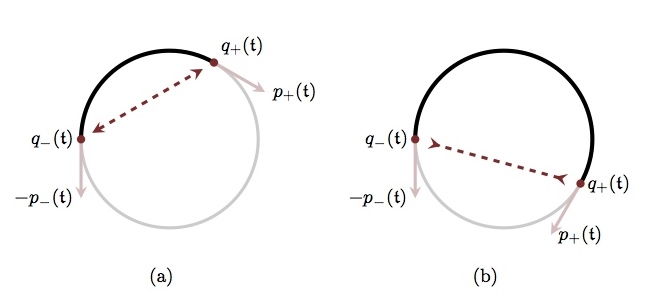
\includegraphics[scale=0.5]{cropped_nuts_image}
  \caption{Visualizing the No-U-Turn sampler. (a) shows a trajectory that is still expanding. (b) shows a trajectory that has started to turn back on itself and expansion stops. Figures come from \cite{betancourt2017conceptual}.}
  \label{nuts-figures}
\end{figure}

Even though the No-U-Turn sampler is named after its termination criterion, which can be described broadly as terminating whenever the trajectory starts to make a u-turn, the criterion itself is a rather crude heuristic that is not justified by any theory. The main advance made by the original NUTS paper \cite{hoffman2014no} is the derivation of a correct and efficient way to construct dynamic leapfrog trajectories by recursively building binary trees. The termination criterion can be further improved, and Stan indeed has adopted NUTS criteria more general than the original and even others where the u-turn aspect is done away with. 

First we look deeper into the No-U-Turn termination criterion. From linear algebra, we know that $x^Ty > 0 $ can be interpreted to say that those two vectors form an acute angle. Then the No-U-Turn criterion 
\begin{align*}
&p_{+}^T (q_+ -q_-) < 0 \Leftrightarrow p_+^T (q_- - q_+) > 0 \\
&p_{-}^T (q_+ -q_-) < 0 \Leftrightarrow -p_-^T (q_+ - q_-) > 0 
\end{align*}
can be explained visually by figures (a) and (b) in \ref{nuts-figures}. Figure (a) shows when the trajectory does not satisfy the terminating criterion and expansion continues. Figure (b) shows when the criterion is satisfied and expansion stops. This idea is generalized in \cite{betancourt2013generalizing}, where the dot product 
\begin{align*}
 p_{+}^T (q_{+} -q_{-})  
 &=p_{+}^T \int_{t=0}^{T} M^{-1}p(t) dt   \\
 &=p_{+}^T M^{-1} \int_{t=0}^{T} p(t)dt \\
 &=(M^{-1} p_{+})^T  \int_{t=0}^{T} p(t)dt \\
 &= p^{\#}_{+}  \int_{t=0}^{T} p(t)dt \\
 &\approx p^{\#}_{+} \sum_{i=0}^n p(t_{k_i}) \\
 &=  p^{\#}_{+} \sum_{z \sim \mathbf{t}} p(z) 
\end{align*} 
is rewritten to accommodate variations of the HMC sampler where non-identity matrices are set as the mass matrix. It is in fact the version of the terminating criterion implemented currently in Stan. Note that in this implementation the criterion is no longer dependent on the position variables $q$. The algorithm for this version of NUTS needs to be adjusted slightly to include a term accumulating the sum of $p$ variables across the subtrees. Pseudocode is provided below.
\SetAlFnt{\footnotesize}
\begin{algorithm}
  	\DontPrintSemicolon
	\SetKwFunction{FBuildTree}{G-BuildTree}

    \KwIn{initial position $q_0$, step size $\epsilon$, joint density $\pi$} 
    Re-sample $p_0 \sim \mathcal{N}(0,\mathbb{I})$ \;
    Initialize $q_{-} = q_0 , q_{+} = q_0 , p_{-} =p_0 , p_+ = p_0, p_+^{\#} = M^{-1}p_+,p_-^{\#} = M^{-1}p_-, p_s = p_0, j =0 ,	q_{\text{next}} = q_0 , s = 1 , w = \pi(q_0,p_0)$ \;
    \While{$s=1$}{
    Choose a direction $v_j \sim \text{Uniform}(\{-1,1\}) $ \;
    \eIf{$v_j = -1$}{
    		$q_-,p_-,-,-,q',s',w',p_{s'} \leftarrow \text{G-BuildTree}(q_-,p_-,v_j,j,\epsilon)$\;
    }{
    		$-,-,q_+,p_+,q',s',w',p_{s'} \leftarrow \text{G-BuildTree}(q_+,p_+,v_j,j,\epsilon)$\;
    }
    \If{$s'=\text{True}$}{
    		With probability $\min(1,\frac{w'}{w})$, set $q_{\text{next}} \leftarrow q_-$\;
    		$p_{s} = p_{s} + p_{s'} $\;
    		$p_+^\# \leftarrow M^{-1} p_{+} $\;
		$p_-^\# \leftarrow M^{-1} p_{-} $\;
    		
    		
    }
    $ w = w + w'$\;
    $ s = s' \mathbb{I}[(q_+ - q_-) \cdot p_-^\# \ge 0 ] \mathbb{I}[(q_+ - q_-) \cdot p_+^\#  \ge 0 ] $\;
    $j = j+1 $ \;
    
    }

\KwRet{$q_{\text{next}}$}

\FBuildTree{$q, p, v, j, \epsilon$}{\;
        \eIf{$j=0$}{
Base case: take one step in direction $v$ \;
$ q' , p' \leftarrow \text{Leapfrog}(q,p,v\epsilon) $ \;
$ w' \leftarrow \pi(q',p') $ \;
$s' = \text{True}$ \;
\KwRet{$q',p',q',p',q',s',w',p_{s'}$} \;

}{
	$p_s = 0 $\;
	$q_-,p_-,q_+,p_+,q',s',w',p_{s'} \leftarrow \text{G-BuildTree}(q,p,v,j-1,\epsilon) $ \;
	
	\If{$s'=\text{True}$}{
		$p_s = p_s + p_{s'}$\;
		\eIf{$v=-1$}{
			$q_-,p_-,-,-,q'',s'',w'',p_{s''} \leftarrow \text{G-BuildTree}(q_-,p_-,v,j-1,\epsilon)$ \;
		}{
			$-,-,q_+,p_+,q'',s'',w'',p_{s''} \leftarrow \text{G-BuildTree}(q_+,p_+,v,j-1,\epsilon)$ \;
		}
		\If{$s''=\text{True}$}{
		
		With probability $\min(1, \frac{w''}{w'+w''})$ , set $q' = q''$. \;
		$p_+^\# \leftarrow M^{-1} p_{+} $\;
		$p_-^\# \leftarrow M^{-1} p_{-} $\;
		$ s' \leftarrow s'' \mathbb{I}[(q_+ - q_- )\cdot p_-^\# \ge 0 ] \mathbb{I}[(q_+ - q_- )\cdot p_+^\# \ge 0 ]$ \;
		$w' \leftarrow w' + w'' $ \;
		$p_{s} = p_{s} + p_{s''} $\;
		
		}
	}
	\KwRet{$q_-,p_-,q_+,p_+,q',s',w',p_{s'}$}\;
}
    }
\caption{Generalized No U-Turn Sampler Update}
\end{algorithm}


The Exhaustive Hamiltonian Monte Carlo (XHMC) termination criterion  relies on a significant amount of differential geometry for its justification\cite{betancourt2016identifying}. Understanding fully the mathematics behind it is beyond the scope of this thesis. From my understanding it is a proxy to monitor the return of a leapfrog trajectory to a neighbourhood around its initial point after having explored the energy level set. With a smaller threshold meant to push the neighbourhood smaller, hence forcing the exploration to continue for longer. Luckily the numerical quantities that needs to be computed are quite easily understood. In the original paper \cite{betancourt2016identifying}, the author demonstrated improved sampling performance over the NUTS criterion as indicated by increased effective sample size on correlated distributions. 

The exhaustive termination criterion is defined as follows: given a threshold $\delta > 0$, terminate trajectory expansion when 
\[  \Bigl |\frac{1}{|\mathbf{t}|} \sum_{z \in \mathbf{t}} \mathbb{P}[z | \mathbf{t}] \frac{dG}{dt}(z) \Bigr | < \delta, \]
where 
\[ \mathbb{P}[z| \mathbf{t}] = \frac{\exp^{-H(z)}}{\sum_{z' \in \mathbf{t}} \exp^{-H(z')}}. \]
The sum can be interpreted as a numerical approximation of an integration over the Hamiltonian flow $\phi_{t}^H(z)$

\[ \lim_{|\mathbf{t}| \rightarrow \infty} \frac{1}{|\mathbf{t}|} \sum_{z \in \mathbf{t}} \mathbb{P}[z | \mathbf{t}] \frac{dG}{dt}(z)  = \lim_{\mathcal{T} \rightarrow \infty} \frac{1}{\mathcal{T}} \int_0^\mathcal{T} dt \frac{dG}{dt} \circ \phi_{t}^H(z) = 0. \]
The function being integrated $\frac{dG}{dt}$, named the virial, is defined as 
\[  \frac{dG}{dt} = \frac{d}{dt}\sum_{i=1}^D q_i p_i.\]
It is a differential-geometric 
quantity designed to measure the return of the trajectory to a neighbourhood containing its initial state. For HMC samplers the virial can be simplified as follows:
\begin{align*}
 \frac{dG}{dt} &= \frac{d}{dt}\sum_{i=1}^D q_i p_i \\
 &= \sum_{i=1}^D p_i \frac{dq_i}{dt} + q_i \frac{dp_i}{dt} \\
 &= \sum_{i=1}^D [M^{-1}p]_i p_i - q_i \frac{\partial V}{\partial q_i} \\
 &= 2 T(p) - q \cdot \frac{\partial V}{\partial q}.\\
\end{align*}
\SetAlFnt{\small}

\begin{algorithm}
  	\DontPrintSemicolon
	\SetKwFunction{FBuildTree}{XHMC-BuildTree}

    \KwIn{initial position $q_0$, step size $\epsilon$, joint density $\pi$} 
    Re-sample $p_0 \sim \mathcal{N}(0,\mathbb{I})$ \;
    Initialize $q_{-} = q_0 , q_{+} = q_0 , p_{-} =p_0 , p_+ = p_0, j =0 ,	q_{\text{next}} = q_0 , s = 1 , w = \pi(q_0,p_0), {ave} = \frac{dG}{dt}(q_0,p_0)$ \;
    \While{$s=1$}{
    Choose a direction $v_j \sim \text{Uniform}(-1,1) $ \;
    \eIf{$v_j = -1$}{
    		$q_-,p_-,-,-,q',s',w',{ave}' \leftarrow \text{XHMC-BuildTree}(q_-,p_-,v_j,j,\epsilon)$\;
    }{
    		$-,-,q_+,p_+,q',s',w',{ave}' \leftarrow \text{XHMC-BuildTree}(q_+,p_+,v_j,j,\epsilon)$\;
    }
    \If{$s'=1$}{
    		With probability $\min(1,\frac{w'}{w})$, set $q_{\text{next}} \leftarrow q_-$\;
    }
     Update ${ave}$ by incorporating ${ave}' $\;
    $ w = w + w'$\;
    $ s = s \mathbb{I}[ \frac{1}{2^j} |{ave} | \ge \delta ] $\;
    $j = j+1 $ \;
    
    }

\KwRet{$q_{\text{next}}$}

\FBuildTree{$q, p, v, j, \epsilon$}{\;
        \eIf{$j=0$}{
Base case: take one step in direction $v$ \;
$ q' , p' \leftarrow \text{Leapfrog}(q,p,v\epsilon) $ \;
$ w' \leftarrow \pi(q',p') $ \;
$ {ave}' \leftarrow \frac{dG}{dt}(q',p') $\;
\KwRet{$q_-,p_-,q_+,p_+,q',s',w',{ave}'$} \;

}{
	$q_-,p_-,q_+,p_+,q',s',w',{ave}' \leftarrow \text{XHMC-BuildTree}(q,p,v,j-1,\epsilon) $ \;
	
	\If{$s'=1$}{
		\eIf{$v=-1$}{
			$q_-,p_-,-,-,q'',s'',w'',ave'' \leftarrow \text{XHMC-BuildTree}(q_-,p_-,v,j-1,\epsilon)$ \;
		}{
			$-,-,q_+,p_+,q'',s'',w'',{ave}'' \leftarrow \text{XHMC-BuildTree}(q_+,p_+,v,j-1,\epsilon)$ \;
		}
		With probability $\min(1, \frac{w''}{w'+w''})$ , set $q' = q''$. \;
		Update $ave$ by incorporating $w'$ and ${ave}'$ \;
		$ s' \leftarrow s''  \mathbb{I}[ \frac{1}{2^j} |{ave} | \ge \delta ] $ \;
		$w' \leftarrow w' + w'' $ \;
	}
\KwRet{$q_{-},p_{-},q_{+},p_{+},q',s',w',{ave}'$}\;
}
    }
\caption{Exhaustive Hamiltonian Monte Carlo Sampler Update}
\end{algorithm}


\section{Adaptive Tuning of Step Size}

The step size $\epsilon$ is arguably the most important tuning parameter for the HMC. Too large of a step size would cause the leapfrog trajectories to diverge. Although the divergence threshold is generally model dependent. For 1-dimensional potential energy function $V(q) = \frac{q^2}{2\sigma^2}$,
that is, normal distributed with variance $\sigma^2$, the threshold can be explicitly computed. Writing out the matrix that encodes the linear mapping from $(q(t),p(t))$ to $(q(t+\epsilon),p(t+\epsilon))$ gives that the mapping is stable if $\epsilon < 2 \sigma$, and diverges otherwise. 

For a general multivariate $q$ with arbitrary potential energy function, equivalent to a general density function, we can approximate the potential energy function with a second order Taylor expansion, so that the $q^2$ term in the Taylor expansion of $V(q)$ has coefficient $\frac{1}{2} \frac{\partial^2 V}{\partial q^2}$  
By matching the two expressions we get 
\[ \sigma \approx \left( \frac{\partial^2 V}{\partial q^2}\right)^{-1/2} \]

Setting $\epsilon$ to that value, we are exactly in the middle of the domain of allowable step sizes, equivalent to half of the boundary limit. While this is a useful heuristic to help one thinks about setting the step size,
care has to be taken to evaluate the second derivative using values of the current parameters, because then the leapfrog steps are no longer reversible; that is since the step size is position dependent, we would get different step sizes at different ends of a trajectory, so when we reverse direction at the other end the trajectory might not be able return to the starting point. This heuristic has been used to guide step size selection in Neal's work on Bayesian neural networks with hierarchical priors.

Now, we describe how the step size is automatically tuned in Stan. First, keep
in mind that the step size is adapted only during the warm-up phase and stays
fixed during the sampling phase. This ensures the correctness of the algorithm
as the induced Markov chain resulted from an adaptive step size may not be
reversible. As a motivation, one way of manual tuning is try to find the step size
$\epsilon'$ that would result in an acceptance probability of $0.65$. The
acceptance probability is an average quantity, calculated as an expectation
over a chain. That is, we try to optimize $\epsilon \in \mathbb{R}$ with respect
to the function 
\[ h(\epsilon) = E_\pi[f(X)|\epsilon]  = \lim_{T \rightarrow \infty} \frac{1}{T}
\sum_{t=1}^T E[f(X_t)|\epsilon] \]
where $f(X_t)$ denotes the acceptance probability for iteration $t$. The
second equality comes from the convergence of the MCMC sampler. This is a
stochastic optimization problem, and Stan uses the dual averaging scheme of
Nesterov to adapt the step size. The dual averaging scheme works in general as
follows. Suppose we are trying to find $x\in \mathbb{R}$ such that $h(x) =
E[H_t|x] = 0$ then we perform the updates 
\[x_{t+1}  = \mu - \frac{\sqrt{t}}{\gamma} \frac{1}{t+t_0} \sum_{i=1}^tH_i; \quad
\bar{x}_{t+1} = \eta_t x_{t+1} + (1-\eta_t) \bar{x}_t \]
where $\mu$ is the target that the $x_t$'s are shrunk towards, $\gamma > 0$ a
parameter that controls the amount of shrinkage, $t_0 \ge 0$ a parameter that
stabilizes the early iterations, and $\eta_t = t^{-\kappa},\kappa>0$  a
step size schedule ensuring convergence. Since $\epsilon>0$, this is technically
a constrained optimization problem, but it can be easily converted into an
unconstrained problem by optimizing for $\log(\epsilon)$ instead. 

\begin{algorithm}
\KwIn{Target Metropolis acceptance rate $\delta$, initial step size $\epsilon_0$, duration of tuning $M^{adapt}$ }

Initialize $\overline{H}_0 = 0, \gamma = 0.05, t_0 = 10 ,\kappa = 0.8 , \mu = \log(10\epsilon_0)$ \;
	
	Calculate acceptance rate $\alpha$ using $\epsilon_0$. \;
\For{$m = 1:M^{adapt}$}{
	 $\overline{H}_m = (1- \frac{1}{m+t_0}) \overline{H}_{m-1} + \frac{1}{m + t_0} (\delta - \alpha) $ \;
	 $\log \epsilon_m = \mu - \frac{\sqrt{m}}{\gamma} \overline{H}_m $ \;
	 $\log \overline{\epsilon}_m = m^{-\kappa} \log \epsilon_m + (1-m^{-\kappa}) \log \overline{\epsilon}_{m-1} $ \;
	
	Update acceptance rate $\alpha$ using $\overline{\epsilon}_m$ \;
	
}

\caption{dual averaging tuning of $\epsilon$ }
\end{algorithm}

Even though there is the dual averaging algorithm for adaptive tuning of the step size, it is still an optimization problem that requires an initialization. Ideally we would an initial $\epsilon$ that this reasonable so as not to waste computational resources. In Stan the original doubling-halving heuristic for initializing the dual averaging optimizer is used. It works by repeatedly doubling or halving the step size, integrating the system for one leapfrog step and evaluating the acceptance rate, until the rate crosses the 50 \% threshold. Hence it avoids starting off with a too large or small step size. 
\begin{algorithm}
Initialize $\epsilon = 1$, momentum $p \sim \mathcal{N}(0,\mathbb{I}) $ \;
$(q',p') \leftarrow \text{Leapfrog}(q,p,\epsilon) $ \;
$a \leftarrow 2 \mathbb{I}[ \frac{\pi(q',p')}{\pi(q,p)} > 0.5 ] -1 $\;
\While{ $(\frac{\pi(q',p')}{\pi(q,p)} )^a > 2^{-a} $}{
	$\epsilon \leftarrow 2^a \epsilon$ \;
	$(q',p') \leftarrow \text{Leapfrog}(q,p,\epsilon) $ \;
}
\KwRet{$\epsilon$}
\caption{find initial $\epsilon$} 
\end{algorithm}

\section{Adaptive Tuning of the HMC Metric}
Stan divides the tuning period into a number of windows of different lengths. The following quantities, followed by their current default values in brackets, are of relevance in this discussion: 

\begin{enumerate}
\item Initial buffer ($n=75$): the first window of the sampling stage, where only the step size parameter is updated by dual averaging .

\item End buffer ($n=50$): the last window of the sampling stage, where the covariance metric is fixed and only the step size is updated and allows it to stabilize.

\item Window size ($n=25$): the base length of interval for updating the covariance metric. 
\end{enumerate}

Both the step size and covariance metric are updated during the tuning stage. And it proceeds as follows: the covariance metric is initialized by the identity matrix and an initial step size is found by the doubling-halving heuristic. Parameter tuning then happens in three stages. The first is the initial buffer, where only $\epsilon $ is updated. In the second stage, both the step size and covariance metric are updated. While $\epsilon$ is updated after every MCMC transition,because the dual averaging procedure only requires an acceptance rate, the covariance metric is updated only after the number of MCMC samples collected equals the current window size. Then compute the empirical covariance and set the metric to its inverse. Then double the window size or increase it to cover the rest of the remaining second stage if doubling is impossible. The third and last stage, which is the end buffer, updates the step size only. 

The algorithm is designed so that the covariance metric is not updated immediately at the start of the tuning stage, because the model might be initialized particularly poorly and hence the initial examples could be misleading. The doubling of window sizes is to allow progressive improvement of the covariance metric. For larger window sizes, the memory requirement for storing all the MCMC samples to estimate the covariance matrix could be prohibitive. Therefore, Stan actually uses an online algorithm for calculating the covariance, whose memory complexity is independent of the window size, which we will discuss in a later section.

\section{HMC-Specific Sampling Diagnostics}

First we describe how Stan uses
divergence to diagnose $\epsilon$'s that are too large. A large constant
is selected, say $Th = 1000$, then after each proposal $(q_i,p_i)$, we compare the
energy value $H(q_i,p_i)$ with that of the previous state $H(q_{i-1},p_{i-1})$,
if $|H(q_i,p_i) - H(q_{i-1},p_{i-1})|> Th$ then a divergence is flagged and the
proposal rejected. This necessarily slows down the the sampler and increases the overall correlation between successive samples. But a divergence should not be interpreted as simply a rejected proposal. The presence of a divergence should call into question the correctness of the samples; the sample
drawn may be biased and hence invalid.
 At the end of the sampling stage, the total number of
divergence indicates potential problem with the chosen step size. Typically the
only response available is to reduce the step size and slow down sampling.
If the problem persists, it may call for reparametrization as the parameter
space may have many sharp edges and steep wells that no step sizes are small
enough to navigate the space.  This is not a diagnostic to be ignored. The recommended practice is zero tolerance for divergent transitions. Even a low number (say $\le 5 $ ) can cause biased samples.

In a static sampler we only need to check for divergence at the end of the leapfrog trajectory. For a NUTS sampler, however, since each state in the trajectory is considered for acceptance when it is first generated, that means we need to check for divergence for each of them. 


The second diagnostic tool that comes with Stan is the Bayesian fraction of
missing information (BFMI) \cite{betancourt2016diagnosing}. It detects a mismatched conditional Hamiltonian
energy function
distribution when compared to the marginal Hamiltonian distribution. 

In a HMC sampler, the leapfrog step is a deterministic process
restricted to exploring a level set determined by the 
initial positions $(q_i,p_i)$ at the start of the trajectory. Given the previous 
state $q_i$, the only randomness introduced in the sampling process comes from the re-sampling of the auxiliary
momentum distribution.  The BFMI is defined as 
\[ \text{BFMI} = \frac{ E_\pi[Var_{\pi_{H|q}}[H|q]]}{Var_{\pi_H}[H]} \]
where $\pi$ is the marginal distribution of $q$ and $\pi_{H|q}$ and $\pi_{H}$
are the conditional and marginal distributions of the Hamiltonian energy
function $H$ respectively.Since the goal is
to explore the energy parameter space, we want the two energy distributions to
 closely match each other, and BFMI allows us to measure that match.

 In practice the expectations must be estimated, but
it is easily done by evaluating the energy function at the values from the
generated Markov chain. Suppose $N+1$ samples are drawn, the estimated BFMI 

\[ \text{E-BFMI} = \frac{\sum_{n=1}^N(H_n-H_{n-1})^2}{\sum_{n=0}(H_n-\bar{H})^2} \]
where $H_n = H(q_n,p_n)$ and $\overline{H}=\frac{1}{N+1}\sum_{n=0}^N H_n$. A low value of $\text{E-BFMI}$ suggests that the auxiliary momentum distribution is
inefficient for sampling. In Stan, the default threshold for low E-BFMI is set to 0.7.

 
\section{Other Sampling Diagnostics}
\label{sec:otherdiag}
Other than divergence and BFMI, Stan also includes MCMC convergence diagnostics that are not specific to HMC samplers. They are the potential scale reduction factor and effective sample size. In the discussion that follows we assume the parameter under investigation is a one dimensional real variable $\psi$, it can be the log-posterior, the variance parameter for a regression model with normal prior, or the posterior mean of a covariate of interest.


The Potential scale reduction factor, also commonly referred to as R hat $\hat{R}$ , can be thought of as the factor by which the scale of the current distribution for $\psi$ might be reduced if the simulations were continued in the limit $n \rightarrow \infty$. This quantity should converge to $1$ as $n \rightarrow \infty$. If $\hat{R}$ is high, $ > 1.1 $, for example, we might want to continue simulation. 

It is defined as follows. Suppose we have $m$ chains each of length $n$, where $\psi_{ij}$ is the $i^\text{th}$ term in chain $j$. Then we have 

\begin{align*}
&B = \frac{n}{m-1} \sum_{j=1}^{m}(\overline{\psi}_{\cdot j} - \overline{\psi}_{\cdot \cdot})^2, \text{ where } 
\overline{\psi}_{\cdot j} = \frac{1}{n} \sum_{i=1}^n \psi_{ij} ,\, \overline{\psi}_{\cdot \cdot} = \frac{1}{m} \sum_{j=1}^m \overline{\psi}_{\cdot j }
 \\
&W = \frac{1}{m} \sum_{j=1}^m s_j^2 , \text{ where }
s_j^2 = \frac{1}{n-1} \sum_{i=1}^n (\psi_{ij} - \overline{\psi}_{\cdot j } )^2.\\
& \hat{\text{var}}^+(\psi|y) = \frac{n-1}{n} W + \frac{1}{n} B \\
& \hat{R} = \sqrt{\frac{\hat{\text{var}}^+(\psi|y)}{W}}. \\
\end{align*}
The Effective Sample Size (ESS) takes into account the autocorrelation inherent in MCMC samples and can be interpreted to represent the equivalent number of independent draws that a set of MCMC draws can replace, for example in calculating expectations and various posterior quantities. The ESS has been computed  differently in the literature. The Stan implementation requires multiple chains and has the advantage that it mitigates the danger of overestimating the ESS when the chain has not converged. It is defined as 
\[n_{\text{eff}}  = \frac{mn}{1 + 2 \sum_{t=1}^\infty \rho_t}, \]
where  $\rho_t$ is the lag at time $t$. The variogram at $t$ 
\[V_t = \frac{1}{m(n-t)} \sum_{j=1}^m \sum_{i=t+1}^n (\psi_{i,j} - \psi_{i-t,j})^2 \]
and the fact $E[(\psi_i - \psi_{i-t})^2] = 2(1-\rho_t)\text{var}(\psi)$ helps to define an estimate for $lag$ at time $t$ 
\[\hat{\rho}_t = 1 - \frac{V_t}{2 \hat{\text{var}}^+}\]
Finally, the ESS is estimated as 
\[\hat{n}_{\text{eff}} = \frac{mn}{1 + 2 \sum_{t=1}^T \hat{\rho}_t}, \]
where $T$ is the first odd positive integer for which $\hat{\rho}_{T+1} + \hat{\rho}_{T+2} $ is negative. It is defined this way because it was observed that for large $T$ the estimates for the lags become too noisy. 
 
\section{Numerical/Implementation Tricks}

Below we list a number of numerical "tricks" that are essential for a successful implementation of a HMC sampler, but usually omitted in the literature. 

First, there is the logsumexp function, which enables numerical stable addition of probability functions on the log scale. It computes
\[ logsumexp(a,b) = \log(\exp(a) + \exp(b) ). \]
While users of traditional MCMC samplers like the Random Walk Metropolis Hastings should be familiar with the idea of computing the Hastings ratio on the log scale to avoid division of probabilities, the NUTS expansion requires updating the probability of the current state by adding the probability from the new subtree. So, instead of doing 
\[ w = w + w' \] 
we would have
\[ \log w = \text{logsumexp}(\log w, \log w' ). \]

\begin{algorithm}
\DontPrintSemicolon
\KwIn{$a,b$}
\KwOut{$c = \log(\exp(a)+ \exp(b)) $}
$s = \max(a,b) $\;
$c = s + \log( \exp(a-s) + \exp(b-s)) $\;

\KwRet{$c$}
\caption{logsumexp}
\end{algorithm}

Similarly, for the Exhaustive Hamiltonian Monte Carlo termination criterion (XHMC) a sum of $\frac{dG}{dt}$ weighted by the probability at the state need to calculated. A numerical stable method calculating both quantities is described below.

\begin{algorithm}
\DontPrintSemicolon
\KwIn{$a_1,\log w_1 , a_2, \log w_2$}
\KwOut{$a = \frac{a_1  w_1 + a_2 w_2}{w_1+w_2} ,\log w = \log (w_1 + w_2)$}

\eIf{$\log w_1 > \log w_2 $}{
	$e = \exp(\log w_1 - \log w_2 ) $\;
	$a = \frac{e \cdot a_1 + a_2}{1+e} $\;
	$\log w = \log w_2 + \log(1+e) $ \;
}{
	$e = \exp(\log w_2 - \log w_1 ) $\;
	$a = \frac{e \cdot a_2 + a_1}{1+e} $\;
	$\log w = \log w_1 + \log(1+e) $ \;
}
\KwRet{$a,\log w$}
\caption{Stable Sum }
\end{algorithm}

The pseudocode for numerically stable versions of the generalized NUTS sampler (GNUTS) and XHMC are given below. Note that it also monitors divergence and rejects automatically any divergent transition.

\begin{algorithm}
	\SetKwFunction{BuildTree}{BuildTree}
	\DontPrintSemicolon

    \KwIn{initial position $q_0$, step size $\epsilon$, joint density $\pi$} 
    Re-sample $p_0 \sim \mathcal{N}(0,\mathbb{I})$ \;
    Initialize $q_{-} = q_0 , q_{+} = q_0 , p_{-} =p_0 , p_+ = p_0, j =0 ,	q_{\text{next}} = q_0 , s = 1 , \log w = H(q_0,p_0)$ \;
    \While{$s=1$}{
    Choose a direction $v_j \sim \text{Uniform}(\{-1,1\}) $ \;
    \eIf{$v_j = -1$}{
    		$q_-,p_-,-,-,q',s',\log w' \leftarrow \text{BuildTree}(q_-,p_-,v_j,j,\epsilon,\log w)$\;
    }{
    		$-,-,q_+,p_+,q',s',\log w' \leftarrow \text{BuildTree}(q_+,p_+,v_j,j,\epsilon,\log w)$\;
    }
    \If{$s'=1$}{
    		With probability $\text{exp}(\min(0,\log w' -\log w))$, set $q_{\text{next}} \leftarrow q_-$\;
    }
    $ w = \text{logsumexp}(w , w')$\;
    $ s = s \mathbb{I}[(q_+ - q_-) \cdot p_- \ge 0 ] \mathbb{I}[(q_+ - q_-) \cdot p_+ \ge 0 ] $\;
    $j = j+1 $ \;
    
    }

\KwRet{$q_{\text{next}}$}\;
\BuildTree{initial position $q$, initial momentum $p$,integration direction $v$,tree depth $j$,step size $\epsilon$,initial Hamiltonian $H_0$} \;
\eIf{$j=0$}{
Base case: take one step in direction $v$ \;
$ q' , p' \leftarrow \text{Leapfrog}(q,p,v\epsilon,H_0) $ \;
$ \log w' \leftarrow H(q',p') $ \;
$ s' = \text{True} \text{ and } \mathbb{I}[\log w' - H_0 > 1000] $\;
\KwRet{$q_-,p_-,q_+,p_+,q',s',\log w'$} \;

}{
	$q_-,p_-,q_+,p_+,q',s',\log w' \leftarrow \text{BuildTree}(q,p,v,j-1,\epsilon,H_0) $ \;
	
	\If{$s'=1$}{
		\eIf{$v=-1$}{
			$q_-,p_-,-,-,q'',s'',w'' \leftarrow \text{BuildTree}(q_-,p_-,v,j-1,\epsilon,H_0)$ \;
		}{
			$-,-,q_+,p_+,q'',s'',w'' \leftarrow \text{BuildTree}(q_+,p_+,v,j-1,\epsilon,H_0)$ \;
		}
		With probability $\text{exp}(\min(0, \log{w''}-\text{logsumexp}(w',w'')))$ , set $q' = p''$. \;
		$ s' \leftarrow s'' \mathbb{I}[(q_+ - q_- )\cdot p^- \ge 0 ] \mathbb{I}[(q_+ - q_- )\cdot p_+ \ge 0 ]$ \;
		$\log w' \leftarrow \text{logsumexp}(w', w'') $ \;
	}
	\KwRet{$q_-,p_-,q_+,p_+,q',s',\log w' $ }\;
}
\caption{Numerically stable No U-Turn Sampler Update with Unity Covariance Metric }
\end{algorithm}

\begin{algorithm}
  	\DontPrintSemicolon
	\SetKwFunction{FBuildTree}{XHMC-BuildTree}

    \KwIn{initial position $q_0$, step size $\epsilon$, energy function $H$} 
    Re-sample $p_0 \sim \mathcal{N}(0,\mathbb{I})$ \;
    Initialize $q_{-} = q_0 , q_{+} = q_0 , p_{-} =p_0 , p_+ = p_0, j =0 ,	q_{\text{next}} = q_0 , s = 1 , \log w = H(q_0,p_0), {ave} = \frac{dG}{dt}(q_0,p_0)$ \;
    \While{$s=1$}{
    Choose a direction $v_j \sim \text{Uniform}(-1,1) $ \;
    \eIf{$v_j = -1$}{
    		$q_-,p_-,-,-,q',s',\log w',{ave}' \leftarrow \text{XHMC-BuildTree}(q_-,p_-,v_j,j,\epsilon,\log w )$\;
    }{
    		$-,-,q_+,p_+,q',s',\log w',{ave}' \leftarrow \text{XHMC-BuildTree}(q_+,p_+,v_j,j,\epsilon,\log w)$\;
    }
    \If{$s'=1$}{
    		With probability $\text{exp}(\min(0,\log w'-\log w)$, set $q_{\text{next}} \leftarrow q_-$\;
    }
     Update ${ave}$ by incorporating ${ave}' $\;
    $ ave, \log w  = \text{stablesum}(ave,\log w,ave',\log w')$\;
    $ s = s \mathbb{I}[ \frac{1}{2^j} |{ave} | \ge \delta ] $\;
    $j = j+1 $ \;
    }
\KwRet{$q_{\text{next}}$}\;

\FBuildTree{$q, p, v, j, \epsilon,H_0$}{\;
        \eIf{$j=0$}{
Base case: take one step in direction $v$ \;
$ q' , p' \leftarrow \text{Leapfrog}(q,p,v\epsilon) $ \;
$ \log w' \leftarrow H(q',p') $ \;
$ {ave}' \leftarrow \frac{dG}{dt}(q',p') $\;
$ s' = \text{True} \text{ and } \mathbb{I}[\log w' - H_0 > 1000] $\;
\KwRet{$q_-,p_-,q_+,p_+,q',s',\log w',{ave}'$} \;

}{
	$q_-,p_-,q_+,p_+,q',s',\log w',{ave}' \leftarrow \text{XHMC-BuildTree}(q,p,v,j-1,\epsilon,H_0) $ \;
	
	\If{$s'=1$}{
		\eIf{$v=-1$}{
			$q_-,p_-,-,-,q'',s'',\log w'',ave'' \leftarrow \text{XHMC-BuildTree}(q_-,p_-,v,j-1,\epsilon,H_0)$ \;
		}{
			$-,-,q_+,p_+,q'',s'',\log w'',{ave}'' \leftarrow \text{XHMC-BuildTree}(q_+,p_+,v,j-1,\epsilon,H_0)$ \;
		}
		With probability $\text{exp}(\min(0, \log w'' -\text{logsumexp}(w',w''))$ , set $q' = q''$. \;
		$ave,\log w \leftarrow \text{stablesum}(ave,\log w,ave',\log w')$ \;
		$ s' \leftarrow s''  \mathbb{I}[ \frac{1}{2^j} |{ave} | \ge \delta ] $ \;
	}
\KwRet{$q_{-},p_{-},q_{+},p_{+},q',s',\log w',{ave}'$}\;
}
}
\caption{Numerically stable Exhaustive Hamiltonian Monte Carlo Sampler Update}
\end{algorithm}




Next we describe the online algorithm used by Stan to calculate the empirical covariance matrix of the target distribution during the tuning stage. It uses the Welford's algorithm \cite{welford1962note}, which only requires storing one vector of the same size as the mean and one matrix of the same dimension as the covariance. 
\begin{algorithm}
\DontPrintSemicolon
\KwIn{current sample counter $t$,accumulator for the mean $m$, accumulator for covariance $m_2$, current sample $x$}

$\delta = x-m$ \;
$m = m + \frac{\delta}{t} $\;
$m_2 = (x-m)\delta^T $ \;
$\mu = m $\;
$\Sigma = \frac{m_2}{t-1} $\;
\KwRet{$m,m_2,\mu,\Sigma$}
\caption{Welford algorithm}
\end{algorithm}

Since HMC only works on unconstrained parameter spaces, any constrained parameters, for example the variance in a normal prior, need to be transformed into unconstrained variables, and transformed back into the original form after the leapfrog steps to calculate acceptance rate. The following identities are useful for coding up the distributions for sampling by HMC.

Suppose $y \ge 0 $ is the original parameter. Then it is first transformed as $X = \text{exp}(y) $ and the log posterior is adjusted by a Jacobian term.
\begin{align*}
p_Y(y) = p_X(f^{-1}(y)) \ |\frac{d}{dY} f^{-1}(y) |\\
p_Y(y) = p_X(\exp(y)) \cdot \exp(y) \\
\log p_Y(y) = \log p_X(\exp(y)) + y \\
\end{align*}
When calculating the ESS, the variogram $V_t$ involves a summation term of the form $\sum_{n=t+1}^N (\theta_{n} - \theta_{n-t})^2$, which can be time-consuming when carried by brute force. From discrete mathematics we know that the Fast Fourier Transform (FFT) can be used to speed up calculation for sums of the form 

\[ \sum_{n=t+1}^N \theta_n \theta_{n-t}.  \]

We can rewrite the sum into a linear combination of the desired form:

\begin{align*}
 \sum_{n=t+1}^N (\theta_{n} - \theta_{n-t})^2 &= \sum_{n=t+1}^N \theta_n^2 - 2 \theta_n \theta_{n-t} + \theta_{n-t}^2  \\
 &= \sum_{n=t+1}^N \theta_n^2 -2 \sum_{n=t+1}^N \theta_n \theta_{n-t} + \sum_{n=t+1}^N \theta_{n-t}^2 \\ 
  &= \sum_{n=t+1}^N  \theta_n^2 \cdot 1  -2 \sum_{n=t+1}^N \theta_n \theta_{n-t} + \sum_{n=t+1}^N 1 \cdot \theta_{n-t}^2 \\
\end{align*}
Finally we discuss a useful heuristic for debugging MCMC samplers. Suppose we have coded a sampler and it seems to run smoothly without a hitch, one might want to use it to sample from a distribution with known mean and covariance, and see if the MCMC samples converge to them in the first and second moments. However, since the empirical mean and covariance will never match exactly the true values, how should we decide if the estimates are close enough?


As an example, suppose we want to sample from a bivariate normal distribution with known mean and covariance matrix. $\mathcal{N}(\mu,\Sigma) $, where 

\begin{displaymath}
\mathlarger{\Sigma} = 
\begin{bmatrix}
\sigma^2_1 &\sigma_{12}^2 \\
\sigma_{21}^2 &\sigma^2_2 \\
\end{bmatrix}.
\end{displaymath}

Given a chain of $n$ MCMC samples $\{x_i\}_{i=1:n}$ generated by the sampler to be tested, we could estimate  the target mean by $ \frac{1}{n-1} \sum_{i=1}^ n x_i$. Since $E[X-\mu] = 0$, and we would expect the generated quantity $\eta= \frac{1}{n-1} \sum_{i=1}^ n x_i -\mu$ to decrease with increasing number of samples. Then we could monitor $\eta$ by comparing it with its Monte Carlo standard error (MCSE) 

\[ \text{MCSE} = \frac{\hat{\sigma}}{\sqrt{n_{\text{eff}}}} \]
where $\hat{\sigma}$ is the estimated standard deviation. By the Central Limit Theorem one would expect  $\eta \in (-\text{MCSE},\text{MCSE})$ with high probability.Similarly we can monitor quantities like $\frac{1}{n-1} \sum_{i=1}^n ({x_i}_1 -\mu_1)^2 - \sigma^2_1,  \frac{1}{n-1}^n \sum_{i=1}^n ({x_i}_1 - \mu_1)({x_i}_2 - \mu_2)^2 $ to assess convergence to the marginal variances and covariance.

One can then construct example models where the mean and covariance are known explicitly, simulate multiple chains and monitor quantities for approximate convergence, in the sense that the empirical estimated quantities differ from their exact quantities by a margin no larger than its MCSE (or its constant multiple .) While this test does not guarantee convergence of the sampler under all circumstances, it is sophisticated enough to detect faulty implementations that leads to non-convergence to the target distribution.

The samplers implemented in this study have been tested on a two dimensional correlated normal distribution with known covariance and a Bayesian logistic regression problem whose posterior covariance is estimated by a long chain generated by Stan.

\chapter{Bayesian Neural Networks}
\section{Introduction to BNNs}

Deep Learning, a field in machine learning which studies multilayered neural network models, has become quite successful in Artificial Intelligence tasks and a lot of research has been, and is being done to improve our understanding of these models and to apply them better and to more fields. See \cite{goodfellow2016deep,lecun2015deep} for a general introduction into the methodology and application of deep learning, and \cite{schmidhuber2015deep} for an in-depth literature review. 

Before there was deep learning, a term which only became popular in the mid 2000s, there were neural networks \cite{bishop1995neural,ripley2007pattern}, which were also hugely popular in the 90s, but eventually the enthusiasim for neural networks cooled off because they were perceived to be too computationally intensive and difficult to scale up. The main reason for this was the difficulty of training neural networks of more than one or two hidden layers. Traditional optimization techniques like stochastic gradient descent with backpropagation did not improve empirical test error for networks with more layers, not until ideas like pre-training to initialize optimization were experimented could we fit "deep" neural networks with more than two hidden layers. This rebooted the field, now rebranded as deep learning, and it was followed by innovations such as using the rectified linear units as activation functions \cite{nair2010rectified} to allow training deep networks without pre-training, and using GPUs to speed up the training process \cite{krizhevsky2012imagenet}, as well as the creation of software libraries like Theano \cite{bergstra2010theano}, Caffe \cite{jia2014caffe}, Tensorflow\cite{tensorflow2015-whitepaper}, and PyTorch \cite{paszke2017automatic}, just to name a few, that make building and training neural network models much easier by automating the backpropogation step with symbolic differentiation \cite{bahrampour2015comparative} and handles the transition between CPU and GPU computation modes. 

First we describe one of the most popular neural network models, the feedforward networks. Suppose we have $n$ observed data points $\{y_i,x_i\}_{i=1}^n$ where $x_i \in
\mathbb{R}^p$ is a $p$-dimensional vector, then a feedforward neural network models the
data as follows:
\begin{align*}
h_1 &= g_1(V_1f_1(W_1 x_i)))\\
h_2 &= g_2(V_2f_1(W_2 h_1))) \\
\vdots& \\
y_i &= g_L(V_Lf_L(W_L h_{L-1})))\\
\end{align*}
where $L$ is the number of layers of the network, $W_j$ a $n_j \times m_{j-1}$
weight matrix, $V_j$ a $m_j \times m_{j-1}$ weight matrix, and each $g_j$,$f_j$
a pair of activation functions that are usually non-linear functions. There are
usually no restrictions on what these activation functions must be other than on
$g_L$ which must match the data type of the $y_i$'s. For example, if $y_i$ are
binary observations then we would like the last output activation function to be a
logistic function so that it maps output strictly to $[0,1]$, just like with the
logistic regression. For a concrete example of a neural network used in practice, see Section \ref{sec:nnmodel}.

Popular activation functions in the classical neural network literature include
the logistic function $f(x) = \frac{1}{1+\text{exp}(-x)} $ and the hyperbolic tangent function $h(x) =  2f(2x)-1$, but in modern deep
learning the rectified linear unit (RELU) has come to dominate the field. It has
a simple form of $g(x)=\max(0,x)$, which is straightforward to do
backpropagation with despite a single point of nondifferentiability, and it was
found to facilitate optimization. It is particularly helpful for
neural network models with many more layers than 2, and it only requires random weight initialization, making it unnecessary to perform pre-training. 

While neural networks can have different numbers of layers and number of hidden
units within each layer, theoretically only one layer is sufficient to
approximate any function as we increase the number of hidden units \cite{hornik1991approximation}. 

For Bayesian neural networks where one puts a Gaussian prior distribution on the weights of the model, it has been shown that for a one-hidden-layer model, the prior converges to a Gaussian process as the number of hidden units converge to infinity \cite{neal2012bayesian}. This gives a neat interpretation of Bayesian neural networks. 

Further work by \cite{gal2015dropout} shows that heuristic training techniques such as dropout \cite{srivastava2014dropout}  are actually doing variational inference with Deep Gaussian Process \cite{damianou2013deep} as its prior, a process where several GPs are stacked one after another. 

The most asymptotically correct way to perform Bayesian inference for BNNs is still MCMC sampling as pioneered in \cite{neal2012bayesian}, in the sense that when the number of MCMC samples goes to infinity they converge to the target posterior distribution, and marginal posterior estimation becomes exact. This is better than alternatives that give biased approximations, such as variational inference \cite{graves2011practical}. In \cite{neal2012bayesian} Neal put a conjugate hiearchical prior on the weights of the network and sampled the weights with HMC and the hyperparameter with block-Gibbs updates. One of his graduate students attempted to sample the weights and hyperparameters jointly with HMC but did not get better performance. Cho \cite{choo2000learning} experimented with a block-Gibbs-HMC hybrid method where each conditional distribution is sampled alternatively by HMC. We experimented with a much simpler alternative for joint sampling and found good results in terms of sample quality. 


Neal found that the windowed HMC sampler improves sampling in general, and also that evaluating the gradient using only a subset of the data would not deterioate performance significantly. We would seek to corroborate those observations in our own experiments.

When assessing convergence of the MCMC samples to the posterior distribution of a Bayesian neural network model, one needs to keep in mind that in general these models have a high number of local modes, usually as an exponential function of the number hidden units \cite{bishop1995neural}. This means we cannot interpret the samples as being drawn from the full posterior distribution, but only from the neighbourhoods containing the local modes that the chains happen to settle around. That means looking at the potential scale reduction (Rhat) for individual weights is probably not that useful because it's not designed to handle multimodal distributions.  

It is still useful to monitor the convergence of the log posterior and of the E-BFMI statistics. Also it can still be useful to monitor the Rhat statistics (see Section \ref{sec:otherdiag}) for the hyperparameter if we can reasonably expect it not to be multimodal, as we can in the case for the variance parameter of a Bayesian neural network.



\section{Sampling for the Hyperparameter}

In Neal's work \cite{neal2012bayesian} he separated the model parameters into groups, and put independent Gaussian-Inverse-Gamma priors on each of them. For example, let $W_{ij}$ be an entry in the weight matrix connecting the input covariates to the hidden units in the first layer. Then, the prior is 
\[W_{ij} \sim \mathcal{N}(0,\sigma^2), \sigma^{-2} \sim \text{Gamma}(a_0,b_0). \]
Assuming the size of weight matrix  $|W|=n $, the posterior distribution for the hyperparameter is once again inverse-Gamma
\[\sigma^{-2}|W,X,y \sim \text{Gamma}(a_1,b_1)\]
\[a_1 = a_0 + \frac{1}{2} n  \]
\[b_1 = b_0 + \frac{1}{2} \sum_{ij} W_{ij}^2 \]
He then proposed alternating between sampling the lower-level weights with HMC and drawing from the conjugate posterior for the hyperparameter exactly. The pseudocode is given below.
\begin{algorithm}
\KwIn{Initial variance $\sigma^2_0$, number of MCMC samples $M$}

\For{$ i = 1:M$ }{
	Sample $W_i \sim p(W|\sigma^2_{i-1},data)$ \;
	$a_1 = a_0 + \frac{1}{2} n $ \; 
	$b_1 = b_0 + \frac{1}{2} \sum_{ij} W_{ij}^2$ \;
	Update $\sigma^2 \sim \text{Inv-Gamma}(a_1,b_1)$ \;
}
\KwRet{$W_{i=1:M}$}
\caption{Blocks-Gibbs Sampler for NN weights and variance}
\end{algorithm}

In Cho's work \cite{choo2000learning}, he experimented with joint sampling of the lower-level weights and hyperparameters. However, since the dual averaging scheme for automatic tuning the step size was not available at the time, he had to rely on the heuristics invented by Neal, which asks for alternate sampling of the conditional distributions in which the step size is dependent on the variables being held constant. He devised a scheme where the leapfrog steps in the joint parameter space have to be done separately for the two groups of parameters. 

A quick note on the parameterization used for the hierarchical prior. The non-centered parametrization (see Section \ref{sec:priors}) is expected to mitigate the posterior correlation between the hyperparameter and the lower-level weights. Reducing posterior correlation is known to help improve sampling efficiency signficantly. We experimented with joint sampling under both parametrizations and found that non-centered parametrization is necessary for meaningful inference. The Hamiltonian sampler also performs better than the block-Gibbs sampler.

\section{Stochastic Gradient Hamiltonian Monte Carlo}
The idea of simulating Hamiltonian dynamics without the Metropolis acceptance step was first experimented in the statistics/machine learning literature by Neal \cite{neal2012bayesian} in a batch HMC sampler for the posterior distribution of a BNN. He found that, with careful selection of the leapfrog step size, the biased samples achieve similar predictive performance as the full MCMC samples. Therefore, it seems to reason that for predictive tasks e.g. regression or classification where observations are abundant, we could 
use a validation set (predictive performance) to select tuning parameters, hoping to trade off a bit of bias for better predictive performance. 

Another trick that helps to speed up the HMC sampler is data subsampling, also denoted partial gradient in Neal's thesis \cite{neal2012bayesian}.
Assuming there are $n$ data points, the potential energy function $V(q)$ can be written as 
\[ V(q) = -\log( \pi(q) \pi(q|data) = -\log(\pi(q)) -\log \pi(q|data) = -\log(\pi(q)) - \sum_{i=1}^n \log \pi(q|data_i) \]
where $\pi(q)$ is the prior density function and $\pi(q|data)$ is the likelihood function. Note that the finite series in the last expression above can be approximated as 
\[ \sum_{i=1}^n \log \pi(q|data_i) \approx \frac{n}{k} \sum_{i \in I} \log \pi(q|data_i) \]
where $I$ is a subset of $\{1,\dots, n\}$ of size $\frac{k}{n}$. 
More practically, if we divide the datapoints into $M$ equally sized subsets. Then for any such subset $S$, the potential energy function can be approximated by 
\[ V(q) \approx    -\log(\pi(q)) + M \sum_{i \in S} \log(\pi(q|data_i)) = \tilde{V}(q) \] Data subsampling and omission of the Metropolis acceptance step are two key features of the stochastic gradient MCMC literature. In an overview of the stochastic gradient MCMC literature \cite{ma2015complete}
the authors summarized it as follows:
 "If the stationary distribution is not the target distribution, a Metropolis-Hastings (MH) correction can often be applied. Unfortunately, such correction steps require a costly computation on the entire
dataset. Even if one can compute the MH correction, if the dynamics do not nearly lead to the correct stationary distribution, then the rejection rate can be high even for short simulation periods $h$. Furthermore, for many stochastic gradient MCMC samplers, computing the probability of the reverse path is infeasible, obviating the use of MH. As such, a focus in the literature is on defining dynamics with the right target distribution, especially in large-data scenarios where MH corrections are computationally burdensome or infeasible.
"

In deep learning, neural networks are usually fitted by stochastic gradient descent (SGD) \cite{ngiam2011optimization}.
This is a first order method like regular gradient descent, except at each weight update a random subset(batch) of data points are sampled to be the  observations, and the sequence of step sizes over the optimization process must decay while satisfying the property
\[ \sum_{t=1}^\infty \epsilon_t = \infty , \sum_{t=1}^\infty \epsilon_t^2 < \infty. \]
Theory from the stochastic optimization literature \cite{robbins1951stochastic} guarantees convergence to a local minimum. However, as per the norm in the optimization literature, the convergence property is usually only provable for easier classes of problems (.e.g. convex, quadratic functions) to which the likelihood of neural network models does not belong. Nonetheless, SGD has the advantage of easy implementation and low memory requirement ($O(D)$), and hence remains the predominant optimization method in deep learning.  

The success of SGD lies in being able to avoid evaluating the full likelihood, which has contribution from each data point, at each update. The problems that neural network models tend to be fitted are usually in the high-sample-size, high-dimensional regime, hence a full evaluation would slow down the algorithm significantly. A stochastic gradient extension to MCMC was first experimented by \cite{welling2011bayesian}, where the author proposed to use the following updates :

\[q_{t+1} = q_t + \frac{\epsilon_t}{2} ( \nabla \log p(q_t) + \frac{N}{n} \sum_{i \in \mathcal{D}} \nabla \log \pi(x_i|q_t) ) + \eta_t , \eta \sim \mathcal{N}(0,\epsilon_t) \]
where $\mathcal{D}$ is a random subset of $\{1,2, \dots, N\}$ of size $n$ sampled at each update of $q$. We assume there are $N$ observations in total. The step sizes are assumed to decay following the constraint stated above for SGD. The authors recommended setting $\epsilon_t = a(b+t)^{-\gamma} $ with $\gamma \in (0.5,1]$.  

The author proved that as the step sizes $\epsilon_t$ goes to $0$ the samples $\{q_t\}$ converge to the Langevin dynamics targeting the posterior distribution. Of course, in practice we set lower bound on $\epsilon_t$ and stop decreasing the step size once it is small enough. Also, the fact the we are not doing the acceptance-rejection step means there will be a bias in our posterior samples, which unlike the samples drawn from a Metropolis-Hastings sampler, does not decrease to $0$ as we sample from the chain longer.


Simulating from the discrete approximation to a Langevin dynamics is the basis
for Langevin Monte Carlo (LMC) or Metropolis adjusted Langevin Algorithm (MALA), which
includes an acceptance-rejection step at each update. This can also be seen as a
special case of HMC where only one leapfrog step is used ($L=1$). It has been
demonstrated that HMC is much more efficient than LMC because it avoids random
walk. This inspires the
stochastic gradient Hamilotian Monte Carlo (SGHMC), 
which extends HMC the way SGLD extends LMC. 


Applying MCMC methods to large datasets often involve two problems. First, evaluating the unnormalized posterior density
\[ \pi(D|q) = \prod_{i=1}^n \pi(x_i|q) \]
 is equivalent to passing through all datapoints, which alone can make the sampling algorithm unacceptably slow since all versions of the Metropolis-Hastings sampler requires such evaluations for proposing new samples. Second, many models that require MCMC samples when a large number of datapoints are available are singular models. Using the terminology of \cite{watanabe2009algebraic}, regular models are models for which the Fisher information matrix is positive definite. They have the property that the Bayesian central limit theorem \cite{le2012asymptotic} holds, that is, when the number of observations goes to infinity the posterior distribution of $q$ converges to a Normal distribution. 
A singular model is defined as a model whose Fisher information matrix is not positive deinfite. A lot of methods designed to scale MCMC \cite{neiswanger2013asymptotically,scott2016bayes} ultimately rely on this asymptotic normality for validity. Bayesian logistic regression is a classical model for which the CLT holds and is used in many papers to demonstrate the effectiveness of newly proposed large-scale MCMC methods. However, the very fact that asymptotic normality holds means there is little added utility to drawing MCMC samples from the posterior distribution, since a normal approximation would suffice. On the other hand, for singular models there is no guarantee that the estimates converge to the target posterior distribution. 

Asympotic normality is also assumed for the application of stochastic gradient MCMC methods to neural network models \cite{welling2011bayesian,chen2014stochastic,ahn2012bayesian,ding2014bayesian,ma2015complete}. Even though neural networks are singular models where the conditions for the central limit theorem do not hold, these methods have shown good predictive performance on a variety of datasets. This is opposite of what one would expect and merits further investigation.


Now we introduce the Stochastic gradient Hamiltonian Monte Carlo (SGHMC). \cite{chen2014stochastic}


\begin{algorithm}
    \caption{Stochastic Gradient HMC}
    \KwData{Input: $\eta,\hat{\beta},\epsilon,\alpha,n,M,L,q_0$}
        Initialize $\theta_0,v_0$ \;
        \For{$t = 1:M$}{
        $q^{0}=q_{t-1}$\;
        $v^{0} \sim \mathcal{N}(0,1) \times \epsilon $ \;
        
        \For{$i = 1:L$}{
        $q^{i} = q^{i-1} + v^{i-1}$ \;
        Sample $z \sim \mathcal{N}(0,2(\alpha-\hat{\beta} \eta))$ \;
        Sample minibatch of size $n$ and calculate $\nabla \tilde{V}(q)$  \;
        $v^{i} = -\eta \nabla \tilde{V}(q) - \alpha v^{i-1} + z$ \;
        }
        
        $q_t = q^{L}$ \;
        $v_t = v^{L}$ \;
        }
\end{algorithm}

Notice that there are two normal distributions being sampled in the algorithm. The first one is the momentum distribution which is the same as the original HMC. The second is a quantitiy designed to account for the uncertainty introduced by replacing the full observed data points by a minibatch. Under simlpifying conditions on the tuning parameters and the subsampling noise model, the SGHMC samples from the target distribution as $\epsilon$ goes to zero. However, those conditions do not usually hold and practice and $\epsilon$ is always fixed at a non-zero value. Nonetheless, these biased samples can be useful if the sampler is tuned carefully.


\section{Priors}
\subsection{Horseshoe Priors}
The horseshoe prior was first proposed by \cite{carvalho2009handling} as a Bayesian counterpart to the frequentist Lasso estimator in high-dimensional statistics. Like the lasso, it shrinks estimates for irrelevant covariates to zero. Compared to alternatives like the Bayesian Lasso \cite{park2008bayesian}, and the spike-and-slab prior \cite{mitchell1988bayesian}, it has the advantage of admitting full HMC sampling because it contains no discrete parameters.

Suppose we have a $D$-dimensional parameter.
\[ \mathbf{\beta} = (\beta_1,\cdots,\beta_D)\]
Then the horseshoe prior for this parameter is defined as
\begin{align*}
 &\beta_j \sim \mathcal{N}(0,\tau^2\lambda^2) \\
 &\lambda_j \sim C^+(0,1),\, j = 1,\dots , D, 
\end{align*}
where $C^+(0,1)$ is a half-Cauchy distribution with mean zero and variance one. The horseshoe prior is usually applied to regression problems where the number of samples were significantly fewer than the number of covariates, which makes it a suitable candidate prior for models that require regularization, like neural networks \cite{ghosh2017model}.

However, the horseshoe prior sometimes causes divergent behaviour during sampling. The regularized horseshoe prior \cite{piironen2017sparsity} fixes this problem and is described below:

\begin{align*}
&\beta_j | \lambda_j, \tau, c \sim \mathcal{N}(0,\tau^2 \tilde{\lambda}_j^2) ,\, \tilde{\lambda}_j^2 = \frac{c^2 \lambda_j^2}{c^2 + \tau^2 \lambda_j^2} \\
&\lambda_j \sim C^+(0,1),\, j = 1,\dots,D\\
&c^2 \sim \text{Inv-Gamma}(2,8) .
\end{align*}
We note that a Cauchy distribution is equivalent to a Student-t distribution of degree 1. A thick-tailed prior like the Student-t is known to cause divergent problems. Therefore, it is often written as a Normal-Inverse Gamma mixture to reduce posterior correlation. That is, $x \sim t_{\nu}(0,1) $ is 
equivalent to 
\begin{align*}
& x \sim \mathcal{N}(0,\sigma^2)\\
&\sigma^2 \sim \text{Inv-Gamma}(0.5,0.5). \\
\end{align*}
We can further reduce correlation by using a non-centered parametrization \cite{piironen2017sparsity}:
\begin{align*}
& x = z * \sigma \\
& z \sim \mathcal{N}^+(0,1)\\
&\sigma^2 \sim \text{Inv-Gamma}(0.5,0.5). \\
\end{align*}
where $\mathcal{N}^+(0,1)$ is a truncated standard normal distribution.
The joint parameter space then becomes $(z,r_1^l,r_2^l,r_1^g,r_2^g) $,
where
\begin{align*}
& z \sim \mathcal{N}(0,1) \\
& \{r_1^l\}_j \sim \mathcal{N}^+(0,1) \, \forall j \\
& \{r_2^l\}_j \sim \text{Inv-Gamma}(0.5,0.5) \, \forall j  \\
& r_1^g \sim \mathcal{N}^+(0,1)  \\
& r_2^g \sim \text{Inv-Gamma}(0.5,0.5)   \\
& \lambda =  r_1^l  r_2^l \\
& \tau = r_1^g  r_2^g \\
& \beta = z  \lambda \tau . \\
\end{align*}
Because the local and global $r_1$ parameters are constrained to be positive, the final unconstrained parameter space is $(z,\log r_1^l,r_2^l,\log r_1^g,r_2^g).$

\subsection{ARD Priors}
Here we would briefly introduce the Automatic Relevance Determination (ARD) priors. It is a general way of assigning priors to the neural network weights that, along with a proper choice of prior, should allow the NNs to self-regulate excess hidden units, and hence obviating the need for choosing the number of hidden units.

An ARD prior puts independent priors of a common distribution on the group of weights entering each hidden unit.
Suppose $W_{i\ell}$ are the weights connecting into the $i^\text{th}$ hidden unit in the $\ell^\text{th}$ layer of a NN. For example, if there are $n$ incoming units connecting to $m$ hidden units and if the prior in question is Normal-Inverse-Gamma, then we have 
\begin{align*}
& W_{i\ell} \in \mathbb{R}^n , \forall i \in \{1,\dots,m\}\\ 
& W_{i\ell} \sim \mathcal{N}(0,\sigma^2) \\
& \sigma_i^2  \sim \text{Inv-Gamma}(a_0,b_0), \forall i \in \{1,\dots,m\} . \\
\end{align*}
\section{Scaled Initialization}
In the neural network literature, the initialization of weights has been observed to influence the final predictive performance of the optimized model. Conventional initializations like the normal distribution with mean 0 and variance 1, and the uniform distribution from 0 to 1 were replaced by scaled distributions whose scale is dependent on the model structure. For example,
\[ W \sim \text{Uniform}(\frac{-1}{\sqrt{N_{in}}},\frac{1}{\sqrt{N_{\text{in}}}}) \]

where $N_\text{in}$ is the number of incoming units from the previous layer. Scaled initializations like this were found to facilitate the propagation the gradients, improve training speed and predictive accuracy \cite{glorot2010understanding}. This motivates us to consider priors of this form. Experiment results will be discussed in Chapter 4.
\section{Model Selection}
In a neural network model there are multiple hyperparameters that has to be selected by
the user. These include the number of hidden layers, the number of hidden
units in each layer, the choice of activation function, the use of
convolutional layers in the case of convolutional neural networks, and the prior
distribution on the weights of the network, just to name a few. Each different combination of these
hyperparameters constitute a model choice. In the neural network literature
usually a holdout test set is used to estimate the test error. The full dataset with observations
$\{\textbf{y},\textbf{x}\}$ is split randomly into a training set
$\{\textbf{y}_{\text{train}}, \textbf{x}_{\text{train}}\}$ and a test set $\{\textbf{y}_{\text{test}},
\textbf{x}_{\text{test}} \}$. Each model is fitted on the training set and its predictive
performance evaluated on the test set.

The model selection procedure above is a special case of cross-validation. Suppose there are $n$ data points. In $k$-fold cross validation,
$k\le n$, the dataset is split into $k$ disjoint subsets, then repeatedly one
subset is used as test set and the remaining sets used as training set. The
extreme case is leave-one-out cross-validation (LOO-CV), where $k=n$. To
calculate the log pointwise predictive density, $\text{lppd}_{\text{loo-cv}}$, we do as
follows. For each split of the $n$ split $\{d_i,d_{-i}\}$, where $d_i$ is the
$i^{\text{th}}$ data point $\{y_i,x_i\}$, and $d_{-i}$ are the $n-1$ remaining data points.
Then
\[ \text{lppd}_{\text{loo-cv}} = \sum_{i=1}^n \log p_{\text{post}(-i)}(d_i), \]
where 
\[p_{\text{post}(-i)(d_i)} = \int p(y_i|x_i,\theta) p(\theta |d_{-i}) d\theta, \]
which is the marginal predictive density of the $i^\text{th}$ data point, with $\theta$
integrated out with respect to the posterior density of $\theta$ having observed
the remaining $n-1$ data points. In practice, the integration is performed
approximately by drawing $S$ samples from $p(\theta|d_{-i})$, denoted
$\{\theta_{-i}^1,\dots, \theta_{-i}^S\}$, and they form the estimate
$\frac{1}{S} \sum_{s=1}^S p(y_i|x_i,\theta_{-i}^s) $.
Then
\[\text{lppd}_{\text{loo-cv}} \approx \sum_{i=1}^n \log (\frac{1}{S} \sum_{s=1}^S
p(y_i|x_i,\theta_{-i}^s))\]
The main obstacle to applying this to model selection for neural networks is the
simulation from $n$ different posterior distribution required, each of these
require tuning and monitoring to ensure low variance of the integral estimate.
For high dimensional distributions such as the posterior distribution of a neural
network, simulation becomes more difficult because of increased computation time as
well as a lack of tools for evaluating convergence of the joint distribution.
Most convergence diagnostics require storing the entire Markov chain, or even
simulating multiple chains,thus further multiplying the the computational burden. Further, it is time-consuming and often unproductive to repeat 10 or 5 times the sampling process  
(in the case of k-fold cross-validation for $k=10$, or $k=5$) when a single sampling session could use up all available memory and computational resources. 
It might not be worth it to obtain a better estimate of the test error if it means shrinking the model to allow repeated sampling sessions.

Holdout cross-validation as currently used in the neural network literature
has higher variance than the k-fold and leave-one-out alternatives and might be
problematic if the sample size is small. It might be
preferable to use an information criterion which requires only simulation from
one posterior distribution, hence reducing the difficulty of assessing convergence and the memory requirement for storing all samples. Traditional information criteria like the
AIC, BIC or DIC rely on the asymptotic normality of the mle for its
justification, which does not hold for non-identifiable (singular) models such
as mixture models, hidden Markov models, and more relevantly here neural network
models. The Watanabe Information Criterion (WAIC) is a recently introduced information criterion that works for
singular models as well. Its justification uses advanced mathematics beyond the
scope of this thesis, notably tools from algebraic geometry and empirical
processes. Hence, we do not attempt to give an intuitive explanation of the
theory and instead take on faith its validity and its asymptotic equivalence to
leave-one-out cross-validation \cite{watanabe2010asymptotic}.

The WAIC can be calculated as follows. Let $\{\theta_1, \dots, \theta_S\}$ be $S$ samples drawn from the posterior distribution $p(\theta|D)$ given all observed data points. Then 

\[\text{WAIC} = \text{lppd} - p_{\text{WAIC}} \]
where 
\[\text{lppd} = \sum_{i=1}^n \log( \frac{1}{S} \sum_{s=1}^S p(y_i|x_i,\theta^s) ) \]
is the computed log pointwise predictive density.And 
\[p_{\text{WAIC}} = \sum_{i=1}^n V_{s=1}^S(\log p(y_i|x_i, \theta^s)) \]
is the effective number of parameters, where $V_{s=1}^S \log(p(y_i|x_i,\theta^s))$ is the empirical variance of the $S$  $\log(p(y_i|x_i,\theta^s))$ for fixed $i$. Note that only $nS$ points need to be stored to calculate the WAIC. $p_{\text{WAIC}}$ can be calculated differently, but here we follow the recommendation in \cite{gelman2014bayesian} and use the formula above.

The WAIC can also be calculated by importance sampling, using the variational distribution as the proposal distribution \cite{yamada2012information}.

Once we have selected a model, we can make predictions about new data using its marginal posterior predictive distribution. That is, given a new data point $\{x_{\text{new}}\}$, we can find its marginal posterior predictive density $p(y_{\text{new}}|D)$ as 
\[ p(y_{\text{new}}|D) = \int p(y_{\text{new}}|x_{\text{new}},\theta) p(\theta|D) d\theta. \]
This integral is usually approximated in practice by drawing from the posterior distribution by MCMC. If this is a classification problem of $C$ classes we would evaluate $p(y_{\text{new}}|D)$ for all $y_{\text{new}}=1,\dots, C$, and if a regression problem a number of points on the domain of the output can be evaluated 
and a prediction made by drawing from the empirical distribution. 
\section{Relation to Stan and PyTorch}

PyTorch \cite{paszke2017automatic} is a deep learning computational framework which contains an automatic differentiation module optimized for neural network models. It also offers the option of GPU computing, which Stan does not provide. What makes it stand out amongst other popular deep learning framework as a prime candidate for implementing the NUTS sampler is that it has a dynamic computational graph framework, which allows easy implementation of recursion and allows backpropogation through it, unlike the static computational graph approach adopted by TensorFlow.

There is concern that single precision might not be enough to maintain accuracy of the Hamiltonian during leapfrog integration, therefore we carried out some experiments comparing the performance of single and double precision numbers on a neural network test problem. Results will be discussed in Chapter 4.


\chapter{Experiments}
\section{Model and Data}
\label{sec:nnmodel}
Having introduced the tools for exploring BNNs and the type of BNNs of interest, in this chapter we will identity the research questions about BNNs and describe the numerical experiments which have been carried out to study them. In the experiments that follow we would focus entirely on classification problems, because that is where neural networks model are employed most and have achieved the most success. Similarly, we would focus on a dataset which is similar in nature to the types of problems usually encountered in the neural network literature, but sufficiently simplified that it does not overtax our computational resources. 

MNIST \cite{lecun-mnisthandwrittendigit-2010} is a benchmark dataset that is arguably the most popular in the machine learning literature. It consists of 60000 images of digits ranging from zero to nine. Each image is of dimension $ 28 \times 28 = 784 $, which already is high enough that it exceeds the memory and time constraint for HMC sampling for a moderate number of hidden units, even in the simplest neural networks with one hidden layer. Therefore, we chose a simplified version of MNIST \cite{scikit-learn} where both the dimension and number of samples are reduced. We compare below the original MNIST and the simplified digits images. The simplified digits has dimension $8 \times 8 = 64 $ and the number of samples is reduced to $1797$. Unless specified, for the following experiments we use the first 500 observations as the training set and the last 500 observations as the test set. While the shapes of the digits could still be made out in the simplified images, the reduced definition blurs classes together so that a 4 might look like a 9 and so on so forth. This should make prediction harder than the original.

\begin{figure}
\begin{tcbraster}[raster columns=5, enhanced, blankest]
\tcbincludegraphics{full_mnist1.png}
\tcbincludegraphics{full_mnist2.png}
\tcbincludegraphics{full_mnist3.png}
\tcbincludegraphics{full_mnist4.png}
\tcbincludegraphics{full_mnist5.png}
\tcbincludegraphics{mnist1.png}
\tcbincludegraphics{mnist2.png}
\tcbincludegraphics{mnist3.png}
\tcbincludegraphics{mnist4.png}
\tcbincludegraphics{mnist5.png}

\end{tcbraster}
\caption{Examples of the digits datasets. The first row contains some examples of the original MNIST digits. The second row contains some simplified digits}
\end{figure}

Unless stated otherwise, all of the experiments that follow use a neural network with one hidden layer, 35 hidden units, and the hyperbolic tangent function as activation function. We omit separate biases weights to simplify the presentation. It does not reduce the representational capacity of the model by too much because one of the hidden units can act as the bias by learning to represent a constant \cite{bishop1995neural}. The simplified model has two groups of weights, namely the input-to-hidden weights of dimension $N_{\text{in}} \times N_{\text{hidden}}$, and the hidden-to-output weights of dimension $N_{\text{hidden}} \times N_{\text{out}} $, where $N_{\text{in}},N_{\text{hidden}},N_{\text{out}}$, are the number of input covariates, hidden units and output units respectively. For example, for the simplified MNIST digits dataset described above, we have $N_{\text{in}} = 64 $ and $N_{\text{out}} = 10 $. Suppose $X,y$ are the training data input and target respectively. A single-hidden-layer neural network with a standard normal prior on its weights would have this unnormalized posterior 

\[ \prod_{i=1}^N p(y,X|W) p(W^{\text{in}})p(W^{\text{out}}) \]
where 
\[p(W^{\text{in}}) = \prod_{k=1}^{N_{\text{in}}}\prod_{j=1}^{N_{\text{hidden}}} \text{exp}\left(- \frac{W_{kj}^{\text{in}} \cdot W_{kj}^{\text{in}}}{2}\right), \]
\[p(W^{\text{out}}) = \prod_{k=1}^{N_{\text{hidden}}}\prod_{j=1}^{N_{\text{out}}} \text{exp}\left(- \frac{W_{kj}^{\text{out}} \cdot W_{kj}^{\text{out}}}{2}\right) \]
are the unnormalized normal prior density functions for the input-to-hidden weights and hidden-to-output weights respectively, and 

\[ p(y_i,X_i) = \prod_{t=0}^9 \hat{\pi}_t^{\mathbb{I}[y_i=t]}, \]
where $\hat{\pi}_t$ is the estimated probability for $X_i$ belonging to class $t$ under the model, computed by 

\[\hat{\pi}_t =   h'(W^{\text{out}}h(W^{\text{in}}X)) \]
where $h$ is the tanh function and $h'$ the softmax function.

For high dimensional models like neural networks with standard normal prior, where no particular one-dimensional quantities could be singled out a priori for monitoring, the usual strategy of monitoring trace plots for diagnosing convergence is infeasible because it would require the user to skim through the trace plots for the thousands of parameters for even a moderately sized network. Therefore, instead we use multiple chains to compute Gelman's effective sample size (ESS) \cite{gelman2014bayesian} and monitor the minimum and median ESS over all parameters. The minimum ESS would indicate to us if any marginal quantities have slow convergence whereas the median would be indicative of the general speed of convergence of the chains as a whole. High ESS is desired as they imply low autocorrelation between samples, which means the Markov chain is moving rapidly across the parameter space and is generating more independent samples.

\section{Comparison with Early Stopping Committees}

In the first experiment we compare a Bayesian neural network to an early stopping committee of neural networks, a frequentist framework which is commonly used as a baseline method. Early stopping is an optimization technique in which training is stopped when the predictive accuracy on a holdout validation set ceases to improve. A group of neural networks initialized with different random seeds, after training by early stopping,  would then combine their predictions by simple averaging. 


The target neural network is a single-hidden-layer network with 35 hidden units, where a standard normal prior has been placed on all weights. An XHMC sampler with a diagonal metric and $\delta = 0.1$ is used to sample from the posterior distribution of the model. The step size and covariance metric are adapted for the first 1000 iterations with the target acceptance rate set to $0.9$. Four parallel chains each of length 2000 are sampled, resulting in 4000 final samples.

We can find the results of the simulation in table \ref{esc}. We see that for smaller sized committees the predictive performance is significantly worse than Bayesian networks. It also reveals the main disadvantage of plain optimization for fitting neural networks, that it is heavily dependent on initialization for good performance. In some experiments we actually found that a single neural network trained by early stopping is enough to match the predictive performance of BNNs, but it requires trying multiple combinations of tuning parameters and initializations. It also requires an extra holdout validation set if we do not want to overfit to the test set. With increasing sizes the bias induced by bad initialization is eventually smoothed out and early stopping committees' predictive accuracies eventually match those of BNNs. 

\begin{table}[]
\centering
\begin{tabular}{@{}rlllll@{}}
\multicolumn{1}{l}{}                            & \multicolumn{5}{c}{Test Error$\%$} \\ \midrule
Method\textbackslash{}Number of ensemble points & 2    & 5   & 10  & 100 & 1000 \\ \midrule
Early Stopping Committee of NNs                 & 91.2  & 88.6 & 47.0 & 51.6 & 19.2  \\ \midrule
BNN                                             & \multicolumn{5}{c}{23.4}        \\ \bottomrule
\end{tabular}
\caption{Compare the predictive accuracy of a Bayesian neural network with early stopping committees of neural networks of different sizes.}
\label{esc}
\end{table}

\section{GNUTS v.s. XHMC}
\label{sec:xhmc}
Since we have established the utility of dynamic HMC for sampling from BNNs, we are now interested in choosing the most suitable termination criterion for the expansion of leapfrog trajectories.  In the following experiment we compare the generalized NUTS termination criterion and the exhaustive termination criterion (XHMC). For both samplers we adapt the step sizes and the diagonal metric and use multiple chains like in the previous experiment. We tested different values of the threshold $\delta$ and found that XHMC is capable of generating samples about as efficiently as GNUTS. Since XHMC is less computationally intensive than the GNUTS, we would recommend the XHMC, however the choice of the threshold $\delta$ still needs to be tuned. For the moment the default $\delta=0.1$ seems to work fine and sampling performance does not seem to be too sensitive to the threshold value. 

\begin{table}[]
\centering
\begin{tabular}{@{}llll@{}}
\toprule
          & Test Error$\%$ & Min ESS & Median ESS \\ \midrule
XHMC $\delta=0.01$  & 25.6       & 681     & 1330       \\ \midrule
XHMC $\delta=0.05$  & 25.8       & 738     & 1346       \\ \midrule
XHMC $\delta=0.1$ & 28.6       & 396     & 1351       \\ \midrule
XHMC $\delta=0.2$ & 23.4       & 822    & 1324        \\ \midrule
GNUTS     & 26.0       & 682     & 1369       \\ \bottomrule
\end{tabular}
\caption{XHMC vs GNUTS}
\label{my-label}
\end{table}


\section{Gibbs Sampling v.s. Joint Sampling for Hyperparameter}
\label{sec:hyperparameter}
Our next research question concerns sampling for the hyperparameter in hierarchical priors. In Neal's work \cite{neal2012bayesian} the BNNs are always endowed with a hierarchical prior, usually normal-inverse-Gamma and sampled by a block-Gibbs sampler. Subsequent attempts to replace the block-Gibbs sampler \cite{choo2000learning} was not successful, and his joint samplers usually generated samples with a high number of divergences. Here we want to find out whether the new automatic tuning techniques for the step size and integration time together with dynamic HMC can overcome these sampling difficulties.

Here, we compare Gibbs sampling with joint sampling for a neural network with a Normal-Inverse-Gamma prior put on the input-hidden weights. A standard normal prior is put on the hidden-out weights. More specifically, we assume 
\[W_{ij} \sim \mathcal{N}(0,\sigma^2), \sigma^{-2} \sim \text{Gamma}(0.5,0.5), \]
which is equivalent to a student-t prior of degree 1 on $W_{ij}$. Both centered (CP) and non-centered (NCP) parametrizations are tried for joint sampling. For the Gibbs sampler, a GNUTS sampler with an identity covariance metric and a conservative step size $\epsilon = 0.01$ is chosen to sample the lower level weights. For joint sampling with both parametrizations, the step sizes and covariance metrics are tuned similarly as in previous experiments.

Focusing only on the variance parameter $\sigma^2$, we see that the CP encounters difficulty during sampling and results in a too low ESS for meaningful inference. In comparison the NCP encounters much less difficulty and has a reasonable ESS relative to the total number of samples. Compared to the  estimates generated by Gibbs sampling, joint sampling gives much higher ESS both for the hyperparameter and the lower-level weights. We tried different step sizes the lower-level weights in the Gibbs sampler but failed to find one that gives decent predictive accuracy and sample efficiency. This simulation shows that joint sampling and automatic step size tuning is an even bigger necessity than previously expected for sampling from BNNs with hierarchical priors.

\begin{table}[]
\centering
\begin{tabular}{@{}lllll@{}}
\toprule
              & Test Error$\%$ & $\sigma^2$ ESS & Min ESS & Median ESS \\ \midrule
Gibbs sampler & 88.4        & 4.38         & 1.29      & 45.3       \\ \midrule
Joint sampler- CP     & 25.8      & 4.86       & 4.69     & 1037         \\ \midrule
Joint sampler - NCP   & 28.4      & 504         & 434     & 1333        \\ \bottomrule
\end{tabular}
\caption{Compare Gibbs Sampling with Joint sampling for the hyperparameter. Note how the centered parametrization has low ESS for $\sigma^2 $ but high ESS in general, translating to good predictive accuracy. }
\label{my-label}
\end{table}

\section{Priors}
\label{sec:priors}
In the following experiments we shall compare the effects of choice of prior on predictive accuracy and sampling efficiency. To keep the presentation simple we chose to use a single-hidden-layer with 35 hidden units. Then we fix the prior on the input-to-hidden weights as the standard normal and vary only the prior on the hidden-to-output weights. For the normal, normal-inv-gamma and horseshoe priors, the application to the weight matrix is simple; we simply consider the matrix as a flattened vector and evaluate the priors as if in regression. This causes no problem even for the hierarchical priors because the hierarchical structure does not involve correlation among the lower level weights. 

The second way to assign such priors to weights is an Automatic Relevance Determination (ARD) type approach, where a local variance is assigned for each hidden unit and one global variance for the entire layer. As an example, suppose the layer in question has $n$ input units and $m$ hidden units. Then, the horseshoe ARD prior can be defined as follows 
\begin{align*}
& W_{i,\cdot} \sim \mathcal{N}(0,\lambda_i^2\tau^2) , \forall i \sim \{1,\dots, m \} \\
& \lambda_i \sim C^+(0,1) \\
& \tau \sim C^+(0,1), 
\end{align*}
where $ W_{i,\cdot}  $ are the weights entering the $i$'th hidden unit. This is how the horseshoe prior was used for model selection in \cite{ghosh2017model}. Similarly we can define the regularized horseshoe ARD prior as 
\begin{align*}
& W_{i,\cdot} \sim \mathcal{N}(0,\tilde{\lambda}_i^2\tau^2) , \, \tilde{\lambda}_j^2 = \frac{c^2 \lambda_j^2}{c^2 + \tau^2 \lambda_j^2}  \forall i \sim \{1,\dots, m \} \\
& \lambda_i \sim C^+(0,1) \\
& \tau \sim C^+(0,1) \\
&c^2 \sim \text{Inv-Gamma}(2,8).
\end{align*}

In the experiments we compared the standard normal prior against a number of hierarchical priors and their ARD variants. We found that while the regularized horseshoe prior performs better than the original horseshoe prior in terms of having zero divergent transitions, neither of the horseshoe priors can be said to induce great sampling efficiency, as both result in models whose posterior distribution are difficult to sample, resulting in low ESS. What's more is that even the Normal-Inverse-Gamma prior does not give better predictive performance than the standard normal prior, which we have already seen in earlier experiments comparing Gibbs sampling to joint sampling for the hyperparameter. 

We observe that the ARD priors in general have better predictive accuracy and \textit{much} better sampling efficiency. For the horseshoe prior in particular, the naive horseshoe application has extremely low mininum ESS it can be considered to be not even converging marginally in some dimensions. We suspect the lower efficiency for the naive horseshoe priors is caused by the higher parameter-to-hyperparameter ratio compared to the ARD versions.
\begin{table}[]
\centering
\begin{tabular}{@{}rrrrrrrr@{}}
\toprule
              & Normal & Normal-Inv-Gamma & Normal ARD     & RHS     & RHS ARD & HS  & HS ARD \\ \midrule
Test Error$\%$    & 23.4    & 26.8    & 24.0& 37.8    & 30.8      & 41.0       & 33.6               \\ \midrule
Min ESS       & 358      & 440   & 574  & 151  & 334     & 4       & 349              \\ \midrule
Median ESS    & 1348      & 1298  & 1220  & 911 & 1356     & 80      & 1354             \\ \midrule
\end{tabular}
\caption{Compare different priors: more complicated hierarchical priors do not necessarily give better predictive accuracy.}
\label{my-label}
\end{table}

\section{SGHMC}
Next we would like to explore stochastic gradient Hamiltonian Monte Carlo. Since it is doubtful that even the full HMC can explore completely the full posterior distribution of a BNN because of its exponential multimodaility, we would not try to compare the empirical distributions of the HMC samples and those of the SGHMC samples directly. Instead we compare the two samplers by their test errors.

The SGHMC has several extra tuning parameters other than the step size $\epsilon$ and number of leapfrogs $L$ that it inherits from the original HMC sampler. To reduce the number of parameters to tune, we fix these parameters ($\alpha=0.01, \hat{\beta}=0$) at the default values used in the experiments even though they are not sufficiently motivated. These are the default values set in the original paper \cite{chen2014stochastic}. The parameters remain to be tuned are $\epsilon,L $ and $\eta$. We generated samples by SGHMC by trying every combination of tuning parameters on a grid of values.


We found that the SGHMC can perform similarly to the HMC although it requires having the right tuning parameter. Because the Metropolis acceptance step is omitted, there is no mechanism to avoid the chain from diverging into a low probability zone in the parameter space. Note that $L=50$ seems to give the best predictive accuracy regardless of the step size, this is puzzling because the $\epsilon$'s span 4 orders of magnitude and thus gives a wide range of integration time $t = \epsilon L$. The role of the learning rate $\eta$ is unclear other than that too large a $\eta$ seems to cause divergence (denoted by NA in the tables) more often. We see that SGHMC can generate samples that have good predictive performance, but there is no clear way to tune all the different hyperparameters other than by a grid search. 


\begin{table}[]
\begin{minipage}{0.5\linewidth}
\centering
\footnotesize
\begin{tabular}{@{}lllll@{}}
\toprule
\multicolumn{5}{c}{Test Error$\%$}                  \\ \midrule
     & $\eta = 0.1$ & $\eta = 0.01$ & $\eta = 0.001$ & $\eta =0.0001$ \\ \midrule
     
$L=10$  & NA       & NA     & 72.2      & 84.4    \\ \midrule
$L=50 $ & 14.8       & 96.6     & 97.6      & 93.4    \\ \midrule
$L=100$  & 34.2      & 20.4    & 47.7     &  89.2  \\ \midrule
$L =200 $ & 46.8      & 37.2   & 92.4      & 87   \\ \bottomrule
\end{tabular}
\caption{SGHMC $\epsilon = 0.1$}
\end{minipage}
\begin{minipage}{0.5\linewidth}
\centering
\footnotesize
\begin{tabular}{@{}lllll@{}}
\toprule
\multicolumn{5}{c}{Test error$\%$}                  \\ \midrule
     & $\eta = 0.1$ & $\eta = 0.01$ & $\eta = 0.001$ & $\eta =0.0001$ \\ \midrule
$L=10$  & NA       & NA     & 68.8     & 84.2    \\ \midrule
$L=50$  & 14.8      & 93.8    & 97.2     & 91.4  \\ \midrule
$L =100$ & 37.2      & 20   & 44.4      & 89.2   \\ \midrule
$L=200 $ & 45.6      & 35.6     & 94      & 85.6   \\ \bottomrule
\end{tabular}
\caption{SGHMC $\epsilon = 0.01$}
\end{minipage}
\begin{minipage}{0.5\linewidth}
\centering
\footnotesize
\begin{tabular}{@{}lllll@{}}
\toprule
\multicolumn{5}{c}{Test Error$\%$}                  \\ \midrule
     & $\eta = 0.1$ & $\eta = 0.01 $& $\eta = 0.001$ & $\eta =0.0001$ \\ \midrule
$L=10$  & NA       & NA     & 68.8      & 89.8    \\ \midrule
$L=50$  & 15.4      & 95.4    & 97.8     & 95  \\ \midrule
$L =100$ & 34.2      & 25.0   & 46.8      & 91   \\ \midrule
$L=200 $ & 54.6      & 46.2     & 97.0      & 88.0   \\ \bottomrule
\end{tabular}
\caption{SGHMC $\epsilon = 0.001$}
\end{minipage}
\begin{minipage}{0.5\linewidth}
\centering
\footnotesize
\begin{tabular}{@{}lllll@{}}
\toprule
\multicolumn{5}{c}{Test Error$\%$}                  \\ \midrule
     & $\eta = 0.1 $ & $\eta = 0.01$ & $\eta = 0.001$ & $\eta =0.0001$ \\ \midrule
$L=10$  & NA       & NA     & 71.6      & 88.0    \\ \midrule
$L=50$  & 15.4      & 93.4    & 96.8     & 88.2  \\ \midrule
$L =100 $& 32      & 21.8   & 45.0      & 88.8   \\ \midrule
$L=200 $ & 53      & 39.4     & 95.4      & 78.4   \\ \bottomrule
\end{tabular}
\caption{SGHMC $\epsilon = 0.0001$}
\end{minipage}
\end{table}


\section{Scaled Priors}
The following experiment investigates whether initializations known to improve predictive accuracy can be used to guide the design of prior for BNN. In this experiment, we compared two normal priors with fixed variances. One is fixed at 1, the other at $\frac{1}{N_{\text{hidden}}}$, the number of hidden units. While we found little difference in their ESS's, the predictive accuracy from the standard normal prior is clearly better. It suggests that the worse predictive accuracy for the scaled priors are not caused by sampling difficulties, but possibly by the prior. It also suggests that the improvement in prediction from using scaled initializations \cite{bengio1994learning} are not the result of having a better prior distribution. More research is needed to provide an explanation.

\begin{table}[]
\centering
\begin{tabular}{@{}llll@{}}
\toprule
            & Test Error$\%$ & Min ESS & Median ESS \\ \midrule
Hidden units = 35 & 23.4 (64.2)        & 358 (683)     & 1348 (1337)       \\ \midrule
Hidden units = 50 & 22.8 (65.0)        & 952 (66)      & 1358 (1348)         \\ \midrule
Hidden units = 65 & 22.0 (69.6)      & 610 (660)      & 1352 (1324)        \\ \bottomrule
\end{tabular}
\caption{Scaled v.s. Unscaled Priors. The figures in brackets show the results for the scaled priors.}

\end{table}

\section{Covariance Adaptation}
Here we explore whether its necessary or indeed useful to condition the HMC by the full covariance matrix of the target distribution. 
We experimented with a number of different priors, where we fixed a neural network model of 35 hidden units in a single hidden layer. We sampled from each posterior distribution 
 and found that not only is adapting the full matrix more time consuming because of the need to multiply by a full mass matrix at every leapfrog step, the samples generated have much higher autocorrelation (equivalent to low ESS) to the point it slows sampling to a halt and destroys any hope of meaningful inference. We attribute this result to the singular nature of neural network models. For each of the prior, we sample from the posterior using the full covariance (dense metric), only the diagonal variances (diagonal metric) and no conditioning (unity metric) respectively. We see that the unity and diagonal metric performs similarly with the diagonal metric giving higher ESSs for the hierarchical priors, and they both take about the same time to compute. Therefore, it suggests that the diagonal metric is most suitable for conditioning the mass matrix, where we get some conditioning by the marginal distributions of the posterior, without incurring the computational cost of a matrix-vector multiplication at each leapfrog step.

\begin{table}[]
\footnotesize
\begin{tabular}{@{}lllll@{}}
\toprule
                     & Test Error$\%$ & Min ESS & median ESS & Compute Time \\ \midrule
Normal               & 67.0 (24.4) [20.6]   & 5 (563) [708] & 17 (1331) [1324]  & 36596 (10165) [11569]     \\ \midrule
Normal-Inv-Gamma     & 86.2 (22.4) [26.0]  & 4 (453) [378]  & 1271 (1348) [1271]    & 38095 (9234) [9158]     \\ \midrule
Normal-Inv-Gamma ARD & 91.2 (23.2) [27.2]  & 4 (370) [140]  & 8 (1295) [1332]    & 74326 (34940) [33212]     \\ \bottomrule
\end{tabular}
\caption{Covariance Adaptation. The figures in round brackets are generated by diagonal metrics, those in square brackets by unity metrics, and those not in brackets by dense metrics. }
\label{my-label}
\end{table}

\section{Number of Layers}
Now we are interested in the impact of the number of layers on sampling efficiency. We know from the neural network literature that deep structures tend to reduce test error. However, there is no empirical studies on the impact of deep hierarchical structures in BNNs, since tradtionally only single-hidden-layer networks were studied.
Here we fix the prior to be a standard normal distribution and vary the number of hidden layers.

Initially we found that increasing the number of layers does reduce the test error, in line with the folk wisdom of the literature. However, for the the models with 4 hidden layers the test errors went up significantly even though the ESSs stay about the same. Since the ESS does not seem to drop precipitously with increasing number layers, the drop in predictive accuracy cannot be attributed to sampling difficulties. In this case it is more likely due to overfitting. It shows that even Bayesian neural networks can overfit, corroborating observations in \cite{gal2015bayesian}.



\begin{table}[]
\centering
\begin{tabular}{@{}lllll@{}}
\toprule
            & Test Error$\%$ & Min ESS & Median ESS & Dimension \\ \midrule
Num Layers = 2 & 16.4    & 284 & 1596       & 3815        \\ \midrule
Num Layers = 3  & 16.8  & 246 & 1418     & 5040        \\ \midrule
Num Layers = 4  & 49.8  & 402 & 1310    & 6265        \\ \bottomrule
\end{tabular}
\caption{Results on the effects of the number of hidden layers. Each layer has 35 hidden units.}
\label{my-label}
\end{table}

\section{Float v.s. Double Precision}
It is important to investigate whether HMC can remain accurate enough for long trajectories that might occur when sampling from BNNs. Since most computations with neural networks are done by graphics processing units (GPU), which only allows single precision, which is 32 bits. Traditionally MCMC computing has always used double precision, which is 64 bits. The loss of precision going from double to single precision is a concern because the stability of the Hamiltonian is critical to the correctness of the algorithm, and we even use divergent transitions to diagnose biased samples. 

 The first experiment looks at the stability of the leapfrog trajectory. The model we used is a single-hidden-layer neural network with 35 hidden units and the normal prior on its weights. First, a number of points ${q_i}$ from the posterior distribution are generated by a sampler in double precision, which are then each augmented by an independent momentum $(p_i)$ drawn from a standard normal distribution. Then the list of $(q_i,p_i)$ points are cast into single precision. The two sets of points are then integrated forward for a fixed number of iterations with a reasonably conservative step size to ensure high acceptance rate, and we compare the difference in Hamiltonian between the start and end point of the trajectory. Denote the Hamiltonian at the end of the double trajectory as $H_d$ and that at the end of the float trajectory as $H_f$. Ideally we would want $H_d-H_f$ to be small if we want the sampler to behave similarly on single and double precision. The initial Hamiltonian does not matter because both trajectories have the same initial state. 

We found that for the normal prior the final states in trajectory differ in energy on average by less than $10^{-5}$ and for the normal-inverse-Gamma prior the difference on the order $10^{-2}$, which translates to at most a difference of 1 $\%$ in the final acceptance rate.


The second experiment investigates whether the loss of precision when adopting single precision would affect the predictive performance. We tested two neural network models with identical structures; both are single-hidden-layer networks with 35 hidden units and the hyperbolic tangent as the activation function. One model has the normal prior on its weights, which is typical of most BNNs used in the literature. The other has a normal-inverse-Gamma prior on the hidden-to-output weights and normal prior on the input-to-hidden-weights. This should be a more difficult model to sample from because of the presence of a hyperparameter which is correlated with most of the lower-level weights. We found that while double precision seems to perform better for the normal prior and single precision better for the hierarchical prior, the difference is not significant enough to be outside of the variance of the estimated test error. 

In both experiments we did not find a significant difference between the two, suggesting that the transition to single precision should not harm predictive accuracy and correctness. 

\begin{table}[]
\centering
\begin{tabular}{@{}rll@{}}
\toprule
\multicolumn{1}{l}{} & Float & \multicolumn{1}{r}{Double} \\ \midrule
Normal               & 27.6   & 25.8                         \\ \midrule
Normal-Inv-Gamma     & 23.2  & 28.8                         \\ \bottomrule
\end{tabular}
\caption{Difference in test error ($\%$) between single and double precision.}
\end{table}

\section{Static v.s. Dynmaic HMC}

First we want to find out whether dynamic HMC is an effective way of sampling from the posterior distribution of a BNN. In Neal's work \cite{neal2012bayesian} he used only static HMC as sampler and relied on using a hierarchical prior in order to use the hyperparameter to set the step size. Therefore, in order to make a fair comparison between static and dynamic HMC for sampling from a BNN with a single-level prior like the standard normal, we decided to use the dual averaging technique introduced in Chapter 2 to tune the step size automatically. 
Secondly, since all dynamic HMC implementations in the literature implicitly embodies a windowed sampler, we would like to separate the effects of dynamic leapfrog trajectories from those of windowed sampling. 
 
In the following experiment we ran two HMC samplers, regular HMC and windowed HMC, over a range of $L$ values, and compare the samples generated by the best $L$ with those generated by dynamic HMC (NUTS). Since the step size is automatically tuned to achieve high acceptance rate, we can assume that most proposals result in acceptance and do not have to worry about the extra bias introduced by an Metropolis acceptance step. Since all samplers have the same target for $\epsilon$, different $L$ values translate to different integration times $t$ by $\epsilon L = t$ .

The model is a single-hidden-layer network with 35 hidden units, with the hyperbolic tangent chosen as the activation function. A standard normal prior is placed on all weights.The step sizes and covariance metrics are tuned automatically as in previous experiments. 

The results show that the static samplers has similar performance as the dynamic sampler, both in terms of predictive accuracy and ESS. Although this may be more indicative of the success of the dual averaging tuning of the step size $\epsilon$ in generating stable leapfrog trajectories. The sampling performance and predictive accuracy seems to be independent of the number of leapfrog steps, and also of the use of the windowed sampler. 
\begin{table}[]
\centering
\begin{tabular}{@{}llll@{}}
\toprule
        & Test Error$\%$ & Min ESS & Median ESS \\ \midrule
$L = 10 $  & 22.8 (22.2)    & 704 (283) & 1061(765)       \\ \midrule
$L = 50 $  & 27.0 (24.2)  & 36 (196)  & 379 (1533)     \\ \midrule
$L = 100  $  & 28.6 (23.8)  & 126 (254)  & 823 (1256)    \\ \midrule
$L = 200  $   & 22.2 (24.0)    & 713 (340)      & 1196 (1204)         \\ \midrule
$L = 500   $ & 23.8  (23.4)       & 345 (693)      & 1245  (1252)        \\ \midrule
Dynamic & 23.4         & 358       & 1348         \\ \bottomrule 
\end{tabular}
\caption{Static v.s. Dynamics HMC. The figures in brackets are generated by windowed HMC}
\label{my-label}
\end{table}

\section{WAIC for Model Selection}

In general, model selection for neural networks is guided by the principle of choosing the model that has the lowest predictive error. In practice this is usually estimated by a holdout test set. However, there are scenarios where we do not have enough data to have a separate holdout test set. In that case we might want to use the WAIC, which does not demand a separate test set but is capable of estimating the true test error asymptotically, at least in theory. In the following experiment we test the WAIC to do just that.

We fix the model to have one hidden layer and vary the number of hidden units. MCMC samples for each model are generated and we compute the estimated WAIC according to the formulae introduced in Chapter 3. The true test error is estimated by a holdout test set.  According to theory, the model with the lowest WAIC should be chosen to minimize predictive error. 


We observe that the model with the lowest WAIC does not match those selected by holdout test error, despite the ESSs indicating decent sample quality.The failure of the WAIC to select the best model might be explained by the poor mixing of the importance sampler when estimating the WAIC, which was noted in a review of predictive checks for Bayesian inference \cite{vehtari2017practical}. It could also be due to the fact that all models being compared actually have comparable test error, when taking into account the natural variance of such an estimate and the Monte Carlo error. Further studies with a larger range of models are required. However, such studies are upper limited by the capacity of the dynamic sampler to sample from larger models, as well as the burden on the computational resources that such expanded studies would require.


\begin{table}[]
\centering
\begin{tabular}{@{}lllll@{}}
\toprule
               & WAIC & Test Error$\%$ & Min ESS & Median ESS      \\ \midrule
Number of Hidden Units = 35    & $3.05 \times 10^4$  & 23.4    & 358 & 1348   \\ \midrule
Number of Hidden Units = 50  & $4.35 \times 10^4$   & 20.4  & 714  & 1342                \\ \midrule
Number of Hidden Units = 75 &$ 6.36 \times 10^4$   & 21.2  & 883  & 1351                 \\ \midrule
Number of Hidden Units = 90 &$ 7.57 \times 10^4$  & 21.2   & 562  & 1359                 \\ \bottomrule
\end{tabular}
\caption{WAIC for model selection}
\label{my-label}
\end{table}


\section{Conclusions}

Experimenting on a simplified MNIST dataset, we found that Bayesian neural networks can achieve about the same and sometimes better predictive accuracy than early stopping committees. The main difference between the two is that early stopping committees need to be manually  tuned to achieve decent accuracy, whereas BNNs can achieve the same with dynamic HMC and automatic tuning of step sizes and covariance metrics. This corroborates previous observations in the literature \cite{neal2012bayesian}. 

Once we can start using BNNs, the challenge becomes finding the best sampler to sample from the posterior distributions. In our experiments we compared static and dynamic HMC samplers. We found that for the static samplers varying the integration time does not seem to influence the predictive accuracy or sample quality, once the step size is chosen so that acceptance rate is kept high. And dynamic HMC is more robust to the choice of tuning parameters than static HMC in terms of sampling efficiency. 

The improvement in sampling efficiency observed by Neal using the windowed HMC sampler \cite{neal2012bayesian} could not be confirmed in our experiment. For our task the windowed HMC sampler does not improve over the regular HMC sampler in terms of ESS as long as the acceptance rate is kept reasonably high. However, it does not generate worse samples either. Perhaps it could still be useful in scenarios where we could not tune for the acceptance rate and the sampler has low acceptance rate.

We then experimented with different termination criteria and found that XHMC can perform as well as GNUTS, and $\delta = 0.1$ seems like a good default threshold value. Although this purely a convenient choice, we note the robustness of the XHMC sampler to the choice of this hyperparamter. We recommend XHMC since it requires fewer computations than GNUTS, which might even scale by a third order factor of the model's dimension if a full covariance metric is used.

We further found that, for dynmaic HMC, automatic tuning of the step size and covariance metric is essential for a robust sampling workflow. Automatic tuning of the step size avoids divergent transitions and tuning the covariance metric improves sampling efficiency by adjusting the scales by their target distribution variances. We found that, however, for BNNs the target distribution is far too complex and cannot be modeled well by a multivariate normal distribution, which the conditioning of the covariance metric implicitly relies on. The dense metric is also more computationally intensive during both the tuning and sampling stage.Hence the diagonal metric should be chosen over the dense metric.

Further comparsion of the Gibbs sampler and joint HMC samplers for the BNNs with hierarchical priors was carried out, and we found that joint sampling by dynamic HMC can be much more efficient for sampling the hyperparmeter. The Gibbs sampler in this instance could not even sample the hyperparameter to any meaningful degree in terms of the ESS. Also, we found that the non-centered parametrizations allowed effective sampling of the hyperparameter, which the centered parameterization was unable to do. This matches the general observations from the Bayesian hierarchical models literature \cite{bernardo2003non}.

Stochastic gradient HMC was investigated and compared with standard HMC for sampling from BNNs, and we found that SGHMC can can give similar performance to HMC but the result is not robust to the choice of tuning parameters. Therefore, it might be worthwhile to try SGHMC if there is enough data for a separate validation set for choosing the tuning parameters. The reduced computational cost of SGHMC means if we choose the right tuning parameter and can accept the unpleasant implications of using a biased sampler, we could achieve better test error than using the full HMC sampler.

On the question of model selection we looked at the WAIC as an alternative to holdout test set for choosing the model which minimizes the predictive error. We were not able to clearly establish the WAIC as a better option for model selection for BNNs than the holdout test set. When faced with insufficient data for creating a new partition into a test set, we do not recommend at the moment using the WAIC for model selection, instead we should collect more data from the data generating distribution.

Now that we have some answers on questions about how to sample from BNNs, we need to choose  the right prior to regulate the weights in typically overparameterized neural network models. We already have experiments showing that the setting the scale of the prior by a multiple of the number of incoming units actually gives worse predictive performance. We further found that automatic relevance determination priors can improve significantly both the predictive accuracy and sampling efficiency, that the regularized horseshoe priors is better than the ordinary horseshoe prior, and that the normal prior is better any of the hierarchical priors test, ARD or otherwise. 

While all the experiments above where conducted in double precision, it is more a choice of convenience than of necessity. We have conducted experiments showing that switching to single precision does not result in a loss of accuracy in the leapfrog trajectories or in the test error computed from the final MCMC samples. This means that we should be able to carry out HMC sampling on GPUs to take advantage of the speed-up without any significant loss of correctness.

Finally, results in this chapter raise more questions about Bayesian neural networks, since some of the results are not what one would expect based some traditional wisdoms about statistics. For example, for overparametrized models where the dimension is much larger than the number of observations, one should use hierarchical priors like the horseshoe to perform regularization. However, our experiments show that such regularization often harms predictive accuracy, even when there is high ESS overall. Also, we found that frequentist predictions could achieve similar predictive accuracy as Bayesian alternatives, although BNNs do seem to be more robust to tuning parameters. These bizarre outcomes need to be explained when we want to investigate claims made about Bayesian neural networks, for example, that they are approximated by stochastic gradient descent \cite{mandt2017stochastic} or other ad-hoc optimization techniques \cite{gal2015dropout,gal2015bayesian}



\chapter{Conclusion}
\section{Conclusion}

	Bayesian neural networks have seen a resurgence with many optimization techniques being interpreted as approximate Bayesian inference. However, these claims were usually made without simulation studies using MCMC for full posterior inference. In this thesis we seek to understand Bayesian inference for BNNs by using the most suitable MCMC methods available to sample from these models. 


In Chapter 2 we looked into the dynamic HMC samplers implemented in Stan and reimplemented them in PyTorch, along with methods for automatically tuning parameters and computing convergence diagnostics. We also provided pseudocode which should help future researchers understand the No-U-Turn sampler as implemented in Stan, since it differs significantly from the original implementation. Special attention needs to be paid to avoid computing probabilities on the original scale to maintain numerical stability.

Then in Chapter 3 we delved into Bayesian neural networks. First we gave a review of the literature, which was mostly the contributions by Neal \cite{neal2012bayesian}. New developments like stochastic gradient Hamiltonian Monte Carlo and scaled initialization in the deep learning literature \cite{chen2014stochastic,bengio1994learning} were introduced and discussed. Finally, we discussed shrinkage priors, their origins in the statistics literature and adaptation for model selection with neural networks. 

The discussions in chapter 2 and 3 provide the motivation for the simulation experiments in Chapter 4. Numerical experiments were conducted to sample from BNNs and compare different strategies. We found that dynamic HMC samplers can sample quite efficiently even from models with complicated hierarchical priors, although these priors do not necessarily improve predictive accuracy. Our main contention is that many of the claims made about BNNs in the deep learning should be scrutinized by further investigation because we found that even with relatively simple models and full MCMC sampling for Bayesian inference the effects of particular new priors do not seem clear, and it seems that sometimes better initialized frequentist models would even beat BNNs sampled by robust, automatically tuned, state-of-the-art HMC samplers.

\bibliographystyle{plain}

\bibliography{test}
\end{document}
